\batchmode
\makeatletter
\def\input@path{{/home/antalcides/MEGA/calculo_I/libro/}}
\makeatother
\documentclass[oneside,english,spanish,2m,twoside,svgnames,x11names,HTML,twoside,12pt]{libro-matua}\usepackage[]{graphicx}\usepackage[]{color}
%% maxwidth is the original width if it is less than linewidth
%% otherwise use linewidth (to make sure the graphics do not exceed the margin)
\makeatletter
\def\maxwidth{ %
  \ifdim\Gin@nat@width>\linewidth
    \linewidth
  \else
    \Gin@nat@width
  \fi
}
\makeatother

\definecolor{fgcolor}{rgb}{0.345, 0.345, 0.345}
\newcommand{\hlnum}[1]{\textcolor[rgb]{0.686,0.059,0.569}{#1}}%
\newcommand{\hlstr}[1]{\textcolor[rgb]{0.192,0.494,0.8}{#1}}%
\newcommand{\hlcom}[1]{\textcolor[rgb]{0.678,0.584,0.686}{\textit{#1}}}%
\newcommand{\hlopt}[1]{\textcolor[rgb]{0,0,0}{#1}}%
\newcommand{\hlstd}[1]{\textcolor[rgb]{0.345,0.345,0.345}{#1}}%
\newcommand{\hlkwa}[1]{\textcolor[rgb]{0.161,0.373,0.58}{\textbf{#1}}}%
\newcommand{\hlkwb}[1]{\textcolor[rgb]{0.69,0.353,0.396}{#1}}%
\newcommand{\hlkwc}[1]{\textcolor[rgb]{0.333,0.667,0.333}{#1}}%
\newcommand{\hlkwd}[1]{\textcolor[rgb]{0.737,0.353,0.396}{\textbf{#1}}}%
\let\hlipl\hlkwb

\usepackage{framed}
\makeatletter
\newenvironment{kframe}{%
 \def\at@end@of@kframe{}%
 \ifinner\ifhmode%
  \def\at@end@of@kframe{\end{minipage}}%
  \begin{minipage}{\columnwidth}%
 \fi\fi%
 \def\FrameCommand##1{\hskip\@totalleftmargin \hskip-\fboxsep
 \colorbox{shadecolor}{##1}\hskip-\fboxsep
     % There is no \\@totalrightmargin, so:
     \hskip-\linewidth \hskip-\@totalleftmargin \hskip\columnwidth}%
 \MakeFramed {\advance\hsize-\width
   \@totalleftmargin\z@ \linewidth\hsize
   \@setminipage}}%
 {\par\unskip\endMakeFramed%
 \at@end@of@kframe}
\makeatother

\definecolor{shadecolor}{rgb}{.97, .97, .97}
\definecolor{messagecolor}{rgb}{0, 0, 0}
\definecolor{warningcolor}{rgb}{1, 0, 1}
\definecolor{errorcolor}{rgb}{1, 0, 0}
\newenvironment{knitrout}{}{} % an empty environment to be redefined in TeX

\usepackage{alltt}
\usepackage[T1]{fontenc}
\usepackage[utf8x]{inputenc}
\setcounter{secnumdepth}{3}
\setcounter{tocdepth}{3}
\usepackage{float}
\usepackage{textcomp}
\usepackage{amstext}
\usepackage{graphicx}

\makeatletter

%%%%%%%%%%%%%%%%%%%%%%%%%%%%%% LyX specific LaTeX commands.
\newcommand{\noun}[1]{\textsc{#1}}

%%%%%%%%%%%%%%%%%%%%%%%%%%%%%% User specified LaTeX commands.
%\usepackage[utf8x]{inputenc}
\usepackage[spanish, es-tabla]{babel}
%\usepackage{makeidx}
\usepackage{imakeidx}
\makeindex[program=truexindy,options=-M texindy -L spanish -C utf8]
%\usepackage[totoc]{idxlayout}
\usepackage{graphicx}
\usepackage{subfigure}
\graphicspath{{ps/}{logo/}{image/}{sections/Figures/}{pdf/}}
%\usepackage{lmodern}
\usepackage{lipsum}
\usepackage{fancyvrb}
\usepackage{cancel}
\raggedbottom %para que no distibuya los espacios verticales en una hoja
\usepackage{pgf}
\usepackage{mathrsfs}
\usetikzlibrary{fit,shapes}
\usepackage{mivenndiagram}
\usepackage{tikz-cd}% diagramas commutativos
\usetikzlibrary{matrix}
\usetikzlibrary{intersections}
\usetikzlibrary{arrows}
\usetikzlibrary{calc}
\usepackage{zahlen}
%\usepackage{fixltx2e}
%\usepackage{mathtools}
%\usepackage{theoremref}
\usepackage{ amsmath,amsfonts,amssymb}
\usepackage{fixltx2e}
\usepackage{mathtools,theoremref,aliascnt}
\usepackage[amsthm, thmmarks]{ntheorem}
\makeatletter
\let\old@thm\@thm
\usepackage{theoremref}
\def\@thm#1#2#3{\def\thmref@currname{#3}\old@thm{#1}{#2}{#3}}
\makeatother

%\MakeRobust{\eqref}
%\mathtoolsset{showonlyrefs=true}
\def\myref#1{\textcolor{ptctitle}{\thesection .\ref{#1}}}
\usepackage[hmargin=2cm,bmargin=3cm,tmargin=4.5cm,centering]{geometry}
\def\yy{\rowcolor{ptcbackground}}
\def\yyy{\rowcolor{gray!50}}
\def\xxx{\rowcolor{ptctitle!50}}
\def\ccc{\cellcolor{ptctitle!50}}
\usepackage{multirow}
\def\maxwidth{8cm}
% Length to control the \fancyheadoffset and the calculation of \headline
% simultaneously
\RequirePackage{hyperref}
\hypersetup{
             linktoc=all,
             hidelinks,
             pdfborder={0 0 0},
            colorlinks=true,
            linkcolor = ptctitle,
            backref=true,
            pagebackref=true,
            hyperindex=true,
            breaklinks=true,
            urlcolor=ocre,
            citecolor = ocre,
            bookmarks=true,
            bookmarksopen=false,
            pdftitle={Title},
            pdfauthor={Author}
                              }
\newlength\FHoffset
\setlength\FHoffset{0.5cm}

\addtolength\headwidth{2\FHoffset}

\fancyheadoffset{\FHoffset}

% these lengths will control the headrule trimming to the left and right 
\newlength\FHleft
\newlength\FHright

% here the trimmings are controlled by the user
\setlength\FHleft{1cm}
\setlength\FHright{0cm}

% The new definition of headrule that will take into acount the trimming(s)
\newbox\FHline
\setbox\FHline=\hbox{\hsize=\paperwidth%
  \hspace*{\FHleft}%
  \rule{\dimexpr\headwidth-\FHleft-\FHright\relax}{\headrulewidth}\hspace*{\FHright}%
}
\renewcommand\headrule{\vskip-.7\baselineskip\copy\FHline}
%%%%%%%%%%%%%%%%%%%%%%%%%%%%%%%%%%%%%%%%%%%%%%%%%%%%%%%%%%
\providecommand\phantomsection{}
%%%%%%%%%%%%%%%%%%%%%%%%%%%%%%%%%%%%%%%%%%%%%%%%%%%%%%%%%
\def\fullwidthcolor#1{\color{#1}\leaders\vrule\hskip\textwidth\hskip-\textwidth\kern0pt}
\def\resetLTcolor{\global\let\zz\zzb}
\def\yy{\rowcolor{ptcbackground}}
\def\yyy{\rowcolor{gray!50}}
\def\xxx{\rowcolor{ptctitle!50}}
\def\ccc{\cellcolor{ptctitle!50}}
\def\yya{\cellcolor{gray!50}}
\def\yyb{\cellcolor{ptcbackground}}
\def\maxwidth{8cm}
%%%%%%%%%%%%%%%%%%%%%%%%%%%%%%%%%%%%%%%%%%%%%%%%%%%%%%%%%%%
\def\firstcircle{(0,0) circle (1.5cm)} 
\def\secondcircle{(45:2cm) circle (1.5cm)}
\def\thirdcircle{(0:2cm) circle (1.5cm)} 
\def\rectangulo{(-2,-2) rectangle (4,3.6)}
\def\fourcircle{(1.1,1) circle (1.5cm)}
\def\fivecircle{(-2,1) circle (1.5cm)}
\def\rect{(-4,-2) rectangle (4,3.6)} 
\def\sixcircle{(1.5,1) circle (1.5cm)} 
\def\sevencircle{(1.1,1) circle (0.8cm)}
%%%%%%%%%%%%%%%%%%%%%%%%%%%%%%%%%% pies de p\'agina %%%%%%%%%%%%%%%%
 \fancyfoot[LE]{\hspace*{-0.2\headwidth}\colorbox{ptctitle!20}{\makebox[\dimexpr 0.6\headwidth-2\fboxsep][r]{\strut\bf\color{ptctitle}C\'alculo diferencial}}%
               \colorbox{zanahoria!60}{\makebox[\dimexpr 0.6\headwidth-2\fboxsep][l]{\strut\bf\color{white}\sffamily\itshape\small\protect\nouppercase{Autor1\hfill Autor2 \hfill Autor3}}}}               
               %%%%%%%%%%%%%%%%%%%%%%
                \fancyfoot[LO]{\hspace*{-0.2\headwidth}\colorbox{ptctitle!20}{\makebox[\dimexpr0.6\headwidth-2\fboxsep][c]{\strut\bf\color{ptctitle}C\'alculo diferencial}}%
               \colorbox{zanahoria!60}{\makebox[\dimexpr0.6\headwidth-2\fboxsep][r]{\strut\bf\color{white}\sffamily\itshape\small\protect\nouppercase{Autor1\hfill Autor2 \hfill Autor3}}}}               
%%%%%%%%%%%%%%%%%%%%%%%%%%%%%%%%%%
%%%%%%%%%%%% conjuntos n\'umericos
\newcommand{\CC}{\mathbb{C}}
%\newcommand{\NN}{\mathbb{N}}
\newcommand{\PP}{\mathbb{P}}
\newcommand{\HH}{\mathbb{H}}
\newcommand{\pp}{\mathbb{\overline{P}}}
\newcommand{\DD}{\mathbb{D}}
\newcommand{\QQ}{\mathbb{Q}}
\newcommand{\RR}{\mathbb{R}}
\newcommand{\ZZ}{\mathbb{Z}}
\newcommand{\EE}{\mathbb{E}}
\newcommand{\TT}{\mathbb{T}}
\newcommand{\XX}{\mathbb{X}}
\newcommand{\der}{\mathcal{D}}
\newcommand{\kk}{\mathcal{K}}
\newcommand{\mm}[1]{{\mathcal{M}\/}(#1)}
\newcommand{\nequiv}{{\equiv \hspace*{-3.7mm}/}}
\newcommand{\capa}[1]{\mbox{{\em Cap\/}}(#1)}
\newcommand{\gra}[1]{\mbox{{\em grad\/}}(#1)}
\newcommand{\sop}[1]{\mbox{{\em supp\/}}(#1)}
\newcommand{\esup}[1]{{\mbox{\rm ess\,sup\/}}#1}
\newcommand{\lqqd}{\hfill $\blacksquare$}
\newcommand{\II}{\mathbb{I}}
\newcommand{\val}[1]{\left|#1\right|}
%\newcommand{\na}{I\! N}
%\newcommand{\re}{I\! R}
{\makeatletter   % dies ist lokal, damit man die Datei wahlweise
                 % mit \input oder mit \documentstyle[...] einlesen kann.
 
\gdef\re{\relax\ifmmode I\hskip -3\p@ R\else
    \hbox{$I\hskip -3\p@ R$}\fi} %Reales
\gdef\na{\relax\ifmmode I\hskip -2.7\p@ N\else
    \hbox{$I\hskip -2.7\p@ N$}\fi} % Naturales
\gdef\en{\relax\ifmmode Z\hskip -4.8\p@ Z\else
    \hbox{$Z\hskip -4.8\p@ Z$}\fi} %Enteros
\gdef\co{\relax\ifmmode C\hskip-4.8\p@\vrule \@height 5.8\p@ \@depth\z@
    \hskip 6.3\p@\else
    \hbox{$C\hskip-4.8\p@\vrule \@height 5.8\p@ \@depth\z@ \hskip 6.3\p@$}\fi}% Complejos
\gdef\ra{\relax\ifmmode Q\hskip-5.0\p@\vrule
          \@height 6.0\p@ \@depth \z@ \hskip 6\p@\else
    \hbox{$Q\hskip-5.0\p@\vrule \@height 6.0\p@ \@depth \z@ \hskip 6\p@$}\fi}% Racionales
\gdef\hz{\relax\ifmmode I\hskip -3\p@ H\else
    \hbox{$I\hskip -3\p@ H$}\fi} % Espacio de Hilbert
\gdef\kz{\relax\ifmmode I\hskip -3\p@ K\else
    \hbox{$I\hskip -3\p@ K$}\fi} % campo K
    \gdef\ir{\relax\ifmmode I\hskip -3\p@ I\else
    \hbox{$I\hskip -3\p@ K$}\fi} % Irracionales}
    %%%%%%%%%%%%%%%%%%%%%%%%%
   % \renewcommand\p@axioma{\thesection.\theaxioma}
   \makeatother
\usepackage{wrapfig}%%% bordear imagen o tabla con texto
\usepackage{siunitx}
\newgeometry{left=2cm,right=2cm,top=2.5cm,bottom=2.5cm}
\newcommand{\inline}{\refstepcounter{equation}~~\mbox{(\theequation)}}%enumera eq inline
\newcommand{\R}{\ensuremath{\mathbb R}}
\newcommand{\Rp}{\ensuremath{{\mathbb R}^{+}}}
\newcommand{\Rm}{\ensuremath{{\mathbb R}^{-}}}
\newcommand{\Rpo}{\ensuremath{{\mathbb R}^{+}_{\,\rm o}}}
\newcommand{\Rmo}{\ensuremath{{\mathbb R}^{-}_{\,\rm o}}}
\newcommand{\Rn}{\ensuremath{{\mathbb R}^{n}}}
\newcommand{\Rx}[1]{\ensuremath{{\mathbb R}^{#1}}}
\newcommand{\N}{\ensuremath{\mathbb N}}
\newcommand{\Z}{\ensuremath{\mathbb Z}}
\newcommand{\nN}{\ensuremath{n\!\in\!\mathbb N}}
\newcommand{\Q}{\ensuremath{\mathbb Q}}
\newcommand{\C}{\ensuremath{\mathbb C}}
\newcommand{\K}{\ensuremath{\mathbb K}} % Cuerpo base
\newcommand{\cont}{\ensuremath{\mathcal{C}}}
\newcommand{\Riemann}{\ensuremath{\mathcal{R}}}%Funciones integrables %Riemann
\newcommand{\A}{\ensuremath{\mathcal{A}}}
\newcommand{\m}{\ensuremath{\Omega}}
\newcommand{\T}{\ensuremath{\mathcal{T}}}        % Topolog�a
\newcommand{\ep}{\ensuremath{\varepsilon\in\Rp}}
\newcommand{\eps}{\ensuremath{\varepsilon}}
\newcommand{\epos}{\ensuremath{\varepsilon>0}}
\newcommand{\dpos}{\ensuremath{\delta>0}}
\newcommand{\irr}{\ensuremath{\mathbb R\!\setminus\!\mathbb Q}}
\newcommand{\ff}{\ensuremath{\varphi}}
\newcommand{\dis}{\displaystyle}
\newcommand{\funcreal}[2]{\ensuremath{\,#1\!:#2\rightarrow \mathbb R\,}}
\newcommand{\cfunc}[2]{\ensuremath{\,#1:#2\rightarrow \mathbb C\,}}
\newcommand{\suc}[1]{\ensuremath{\{#1\}}}
\newcommand{\sucsub}[2]{\ensuremath{\{#1_{#2}\}}}
\newcommand{\sucn}[1]{\ensuremath{\{#1_{n}\}}}
\newcommand{\sucm}[1]{\ensuremath{\{#1_{m}\}}}
\newcommand{\sucN}[2]{\ensuremath{\,\{#1_{#2}\}_{#2\in\mathbb N}}}
\newcommand{\sucNo}[2]{\ensuremath{\,\{#1_{#2}\}_{#2\in\mathbb N_{\rm o}}}}
\newcommand{\parcial}[1]{\ensuremath{\{#1_{\sigma(n)}\}}}
\newcommand{\parcialf}[1]{\ensuremath{\{#1_{varphi(n)}\}}}
\newcommand{\Suma}[1]{\mbox{${\displaystyle \sum_{#1=-\infty}^\infty}$}}
\newcommand{\suma}[1]{\mbox{${\displaystyle \sum_{#1}}$}}
\newcommand{\sumaf}[2]{\mbox{${\displaystyle \sum_{#1}^{#2}}$}}
\newcommand{\sumainf}[1]{\mbox{${\displaystyle \sum_{#1}^{\infty}}$}}
\newcommand{\sumasubn}[1]{\mbox{${\displaystyle \sum_{n\geqslant #1}}$}}
\newcommand{\serie}[1]{\mbox{${\displaystyle \sum_{n\geqslant 1}#1\,}$}}
\newcommand{\serien}[1]{\mbox{${\displaystyle \sum_{n\geqslant 1}\!#1_n\,}$}}
\newcommand{\serieno}[1]{\mbox{${\displaystyle \sum_{n\geqslant 0}\!#1\,}$}}
\newcommand{\Suman}[1]{\mbox{${\displaystyle \sum_{n=1}^{\infty}\!#1_n\,}$}}
\newcommand{\ser}[1]{\mbox{$\{#1_1+#1_2+\cdots+#1_n\!\}$}}
\newcommand{\serabs}[1]{\mbox{$\{|#1_1|+|#1_2|+\cdots+|#1_n|\!\}$}}
\newcommand{\armd}{\mbox{$\dis\bigg\{1+\frac{1}{2}+\cdots+\frac{1}{n}\bigg\}$}}
\newcommand{\arm}{\mbox{$\{1+1/2+\cdots+1/n\}$}}
\newcommand{\Arm}{\mbox{$1+\dfrac{1}{2}+\cdots+\dfrac{1}{n}$}}
\renewcommand{\en}{\!\in\!}
\newcommand{\bcapn}[1]{\mbox{$\dis\bigcap_{#1\in\mathbb N}$}}
\newcommand{\bcupn}[1]{\mbox{$\dis\bigcup_{#1\in\mathbb N}$}}
\newcommand{\bcupzn}[1]{\mbox{$\dis\bigcup_{#1\in\mathbb Z}$}}
\newcommand{\integ}[3]{\mbox{$\int_{#1}^{#2}#3\,$}}
\newcommand{\dispinteg}[3]{\mbox{${\displaystyle \int_{#1}^{#2}\!#3\,}$}}
\newcommand{\vac}{\mbox �}
\newcommand{\fin}{~\hfill \textcolor{myblue!75!black}{$\Box$}\newline\smallskip}
\newcommand{\sskip}{\vspace{2mm}}
\newcommand{\bskip}{\vspace{3mm}}
%\newcommand{\dem}{\noindent{\textbf{\textcolor{myblue!75!black}{Demostraci\'on}}.\ }}
%\newcommand{\sol}{\noindent{\textbf{\textcolor{myblue!75!black}{Soluci\'on.}}\ }}
\newcommand{\hecho}{\noindent{~\hfill\Large\color{red}{\Smiley{}} }}% usa marvosym
\DeclareMathOperator{\dist}{dist}
\DeclareMathOperator{\sen}{sen}
\DeclareMathOperator{\tg}{tg}
\DeclareMathOperator{\arctg}{arctg}
\DeclareMathOperator{\arcsen}{arcsen}
\DeclareMathOperator{\senh}{senh}
\DeclareMathOperator{\argsenh}{argsenh}
\DeclareMathOperator{\argcosh}{argcosh}
\DeclareMathOperator{\Arccos}{Arccos}
\DeclareMathOperator{\Arcsen}{Arcsen}
\DeclareMathOperator{\Arctg}{Arctg}
\DeclareMathOperator{\cotg}{cotg}
\DeclareMathOperator{\cosec}{cosec}
\DeclareMathOperator{\tgh}{tgh}
\DeclareMathOperator{\argtgh}{argtgh}
\DeclareMathOperator{\argcosech}{argcosech}
\DeclareMathOperator{\Arg}{Arg}
\DeclareMathOperator{\arcsec}{arcsec}
\DeclareMathOperator{\arccosec}{arccosec}
\DeclareMathOperator{\argsech}{argsech}
\newcommand{\enC}[1]{\ensuremath{#1\!\in\!\mathbb C}}
%\DeclareMathOperator{\re}{Re}
\DeclareMathOperator{\im}{Im}
\DeclareMathOperator{\Log}{Log}
\newcommand{\conj}[1]{\mbox{$\overline{\rule{0mm}{1.8mm}#1}$}}
\newcommand{\Lim}[3]{\mbox{$\displaystyle{\lim_{#2\to #3}#1}$}}
\newcommand{\limlft}[3]{\mbox{$\dis{\lim_{\substack{#2\to #3\\ #2\,<\,#3}}#1}$}}
\newcommand{\limrgt}[3]{\mbox{$\dis{\lim_{\substack{#2\to #3\\ #2\,>\,#3}}#1}$}}
\newcommand{\Dfa}{\mbox{$f^{\,\prime}(a)$}}
\newcommand{\Dfka}{\mbox{$f^{\,(k)}(a)$}}
\newcommand{\Dfna}{\mbox{$f^{\,(n)}(a)$}}
\newcommand{\llfrac}[2]{\mbox{$\left\{ \dfrac{#1}{#2}\right\}$}}
\DeclareMathOperator{\e}{e}
\newcommand{\tl}{\mbox{$^{\mspace{2mu}\prime}$}}
\newcommand{\tlo}{\mbox{$^{\prime}$}}
\newcommand{\fder}[1]{\mbox{$#1^{\,\prime}$}}
\newcommand{\Derdos}[2]{\mbox{$#1^{\,\prime\prime}(#2)$}}
\newcommand{\derpar}[2]{\mbox{$\dfrac{\partial #1}{\partial #2}$}}
\newcommand{\derpardos}[2]{\mbox{$\dfrac{\partial^{2}\! #1}{\partial #2^{2}}$}}
\newcommand{\scd}{\mbox{$^{\,\prime\prime}$}}
\newcommand{\Der}[2]{\mbox{$#1^{\,\prime}(#2)$}}
\newcommand{\Derk}[2]{\mbox{$#1^{\,(k)}(#2)$}}
\newcommand{\Dern}[2]{\mbox{$#1^{\,(n)}(#2)$}}
\newcommand{\escalar}[2]{\ensuremath{\left\langle #1\,\big |\, #2\right\rangle}}
\newcommand{\norm}[1]{\ensuremath{\lVert#1\rVert}}
\newcommand{\partx}[1]{\ensuremath{\dfrac{\partial #1}{\partial x}}}
\newcommand{\party}[1]{\ensuremath{\dfrac{\partial #1}{\partial y}}}
\newcommand{\partz}[1]{\ensuremath{\dfrac{\partial #1}{\partial z}}}
\newcommand{\partxx}[1]{\ensuremath{\dfrac{\partial^2 #1}{\partial x^{2}}}}
\newcommand{\partyy}[1]{\ensuremath{\dfrac{\partial^2 #1}{\partial y^2}}}
\newcommand{\partxy}[1]{\ensuremath{\dfrac{\partial^2 #1}{\partial x
\partial y}}}
\newcommand{\partyx}[1]{\ensuremath{\frac{\partial^2 #1}{\partial y
\partial x}}}
\newcommand{\partone}[2]{\ensuremath{\dfrac{\partial #1}{\partial #2}}}
\newcommand{\partwo}[2]{\ensuremath{\dfrac{\partial^2 #1}{\partial #2^2}}}
\newcommand{\partonetwo}[3]{\ensuremath{\dfrac{\partial^2 #1}{\partial #2\partial #3}}}
\newcommand{\setbig}[1]{\big\{ #1 \big\}}
\newcommand{\set}[1]{\left\lbrace #1 \right\rbrace}
\renewcommand{\ge}{\geqslant}
\renewcommand{\le}{\leqslant}
%\newcommand{\inte}[1]{\overset{\circ}{#1}}      % Interior de un conjunto
\newcommand{\cajadoble}{\psdblframebox[linewidth=.6pt]}
\newcommand{\azul}{\color[rgb]{0,0,1}}
\newcommand{\negro}{\color[rgb]{0,0,0}}
\newcommand{\rojo}{\color[rgb]{1,0,0}}
\newcommand{\lra}[1]{\ensuremath{\left\langle #1 \right\rangle}}
\newcommand{\modulo}[1]{\left\lvert{#1}\right\rvert}
\newcommand{\abs}[1]{\lvert{#1}\rvert}  % Valor absoluto
\newcommand{\norma}[1]{\left\|{#1}\right\|}         % Norma
\newcommand{\df}[1]{\,\mathrm{d}#1\,}               % Diferencial
\newcommand{\derivada}[2]{\dfrac{\df{#1}}{\df{#2}}}  % Derivada de #1 respecto de #2
\newcommand{\derivadados}[2]{\ensuremath{\dfrac{\mathrm{d}^2 #1}{\mathrm{d}#2^2}}}
\newcommand{\derivadatres}[2]{\ensuremath{\dfrac{\mathrm{d}^3 #1}{\mathrm{d}#2^3}}}
\newcommand{\derivadan}[2]{\ensuremath{\dfrac{\mathrm{d}^n #1}{\mathrm{d}#2^n}}}
\newcommand{\derparcial}[2]{\ensuremath{\dfrac{\partial #1}{\partial
#2}}}
\DeclareMathOperator{\fr}{Fr}         % Frontera
\renewcommand{\leq}{\leqslant}
\renewcommand{\geq}{\geqslant}
\newcommand{\mb}{\mathbf}
\DeclareMathOperator{\senc}{senc}
\DeclareMathOperator{\sgn}{sgn}
\renewcommand{\Re}{\re}
\renewcommand{\Im}{\im}
\newcommand{\ms}{\mspace}
\newcommand{\msi}{\mspace{1mu}}
\newcommand{\msii}{\mspace{2mu}}
\newcommand{\msiii}{\mspace{3mu}}
\newcommand{\into}{\int_0^\infty}
\newcommand{\nw}[1]{\ensuremath{\overset{\centerdot}{#1}}}
\newcommand{\nww}[1]{\ensuremath{\overset{\centerdot\centerdot}{#1}}}
\newcommand{\func}[2]{\mbox{$\,#1:#2\rightarrow \R\,$}}
\newcommand{\vectorx}{\ensuremath{(x_1,x_2,\dots,x_n)}}
\newcommand{\vectory}{\ensuremath{(y_1,y_2,\dots,y_n)}}
\newcommand{\vectorz}{\ensuremath{(z_1,z_2,\dots,z_n)}}
\newcommand{\vectora}{\ensuremath{(a_1,a_2,\dots,a_n)}}
\newcommand{\vectorb}{\ensuremath{(b_1,b_2,\dots,b_n)}}
\newcommand{\vectorc}{\ensuremath{(c_1,c_2,\dots,c_n)}}
\newcommand{\esc}[2]{\ensuremath{\left\langle #1\, \mathbf{|}\,#2 \right\rangle}}
\newcommand{\vx}{\ensuremath{\mathbf{x}}}
\newcommand{\vy}{\ensuremath{\mathbf{y}}}
\newcommand{\vz}{\ensuremath{\mathbf{z}}}
\newcommand{\va}{\ensuremath{\mathbf{a}}}
\newcommand{\vb}{\ensuremath{\mathbf{b}}}
\newcommand{\vc}{\ensuremath{\mathbf{c}}}
\newcommand{\vu}{\ensuremath{\mathbf{u}}}
\newcommand{\vv}{\ensuremath{\mathbf{v}}}
\newcommand{\vw}{\ensuremath{\mathbf{w}}}
\newcommand{\vr}{\ensuremath{\mathbf{r}}}
\newcommand{\vf}{\ensuremath{\mathbf{F}}}
\newcommand{\vn}{\ensuremath{\mathbf{n}}}
\newcommand{\vt}{\ensuremath{\mathbf{t}}}
\newfont{\esclar}{cmmib10}% El punto para el producto escalar
\newcommand{\dt}{\esclar\mbox{\symbol{58}}}
\newfont{\mifuente}{cmbsy10}% El infinito es  el car�cter 49 en esta fuente.
\newcommand{\infinity}{\mifuente\mbox{\symbol{49}}} %S�mbolo infinito
\newfont{\adornos}{fourier-orns}% ornamentos
\newcommand{\volutaleft}{\adornos\mbox{\symbol{91}}} % adorno voluta
\newcommand{\volutaright}{\adornos\mbox{\symbol{92}}} % adorno voluta
\newcommand{\florleft}{\adornos\mbox{\symbol{98}}} % adorno flor
\newcommand{\florright}{\adornos\mbox{\symbol{99}}} % adorno flor
\newcommand{\manoright}{\adornos\mbox{\symbol{116}}} % adorno mano izquierda
\newcommand{\manoleft}{\adornos\mbox{\symbol{117}}} % adorno mano derecha
\newfont{\librotex}{manfnt}% figuras del libto de Knuth "The TeX Book"
\newcommand{\curvasr}{\librotex\mbox{\symbol{126}}} % curvas peligrosas dcha
\newcommand{\curvasl}{\librotex\mbox{\symbol{127}}} % curvas peligrosas izqda
\newfont{\noesta}{psyr}
\renewcommand{\notin}{\noesta\mbox{\symbol{207}}}
%\newfont{\implicadcha}{mtsyt}
\renewcommand{\Longrightarrow}{\implicadcha\mbox{\symbol{144}}}
\newcommand{\raiz}{\mbox{$\sqrt{a x^{2} + b x + c}\,$}}
\newcommand{\rac}[1]{\mbox{$\sqrt{#1}\,$}}
\makeatletter
\patchcmd{\@eqnnum}{\normalcolor}{\color{zanahoria}}{\typeout{eqnnum patch: OK!}}{\typeout{eqnnum patch: Oh, dear!}}
\makeatother
\newcommand{\arco}[2][30pt]{\overset{\tikz \draw[rotate=60,line width=1pt]
 (#1,0pt) arc (0:60:#1);}{#2}}
%%%%%%%%%%%%%%%%%%%%%%%%%%%%%%%%%%%%%%%%%%%%%%%%%Nota y soluci�n%%%%%%%%%%%%%%%%%%%%%%%%%%%%%%%%%%%%%%%%%%%%%%%%%%%%%%%%%%%%%%%%
%\newcommand{\solucion}{\colorbox{black}{\color{white}{Soluci�n:}}}
%\newcommand{\nota}{\colorbox{teal!20!white}{\color{black}{Nota:}}}
\newcommand{\degre}{\ensuremath{^\circ}}
\newcommand{\grado}{\ensuremath{^\circ}}
%\newfont{\wasi}{wasy10}% para incluir integrales rectas
%\newcommand{\varint}{\wasi\mbox{\symbol{119}}} %NO funciona
%\newcommand{\rac}[1]{\mbox{$\sqrt{\rule{0mm}{3.2mm} #1}\,$}}
%\newcommand{\raiz}{\mbox{$\sqrt{\rule{0mm}{3.2mm} ax^{\,2}+bx+c}\,$}}
%\newfont{\noestados}{usyr}
%\renewcommand{\notin}{\noestados\mbox{\symbol{207}}}
%\newfont{\sonrisa}{wasy10}% para incluir el smiley
%\newcommand{\smiley}{\sonrisa\mbox{\symbol{44}}}
%\newfont{\sonrisagrande}{umvs}% fuente marvosym
%\newcommand{\smileygrande}{\sonrisagrande\mbox{\Large\symbol{169}}}
%\renewcommand{\Longrightarrow}{\largaimplica\mbox{\symbol{222}}}
% Espacio de las funciones %continuas
%\newcommand{\h}{\ensuremath{\mathcal{H}}}        % Funciones holomorfas
%\newcommand{\M}{\ensuremath{\mathcal{M}}}   % Transformaciones de M�bius
%\newcommand{\F}{\ensuremath{\mathcal{F}}}
%\newcommand{\Cc}{\ensuremath{\mathscr{C}}}       % Conjunto de %rectas-circunferencias
%\newcommand{\Ca}{\ensuremath{\widehat{\mathbb C}}} % El cuerpo de los %complejos %ampliado con el infinito %\DeclareMathOperator{\rot}{rot} \DeclareMathOperator{\diver}{div}
%\renewcommand{\pi}{\,\piup} % requiere cargar txfonts
%\newcommand{\tf}[1]{\ensuremath{\mathscr{F}\!#1}}
%\newcommand{\tfi}[1]{\ensuremath{\mathscr{F}^{\,-1}\!#1}}
%\newcommand{\itf}[1]{\ensuremath{\check{#1}}}
%\newcommand{\tla}[1]{\ensuremath{\mathscr{L}\!#1}}
%\newcommand{\tli}[1]{\ensuremath{\mathscr{L}^{\,-1}\!#1}} %\DeclareMathOperator{\res}{Res}
%\DeclareMathOperator{\ind}{Ind}% �ndice respecto de una curva
%\renewcommand{\emptyset}{\vac}  % Para redefinir el s�mbolo del conjunto vac�o
%\renewcommand{\int}{\varint}    % para usar el s�mbolo de integral del paquete %wasysym %\newcommand{\csuma}{\overset{\centerdot}{+}}        % Yuxtaposici�n de curvas
%\newcommand{\copuesta}{\overset{\centerdot}{-}}     % Curva opuesta
%\renewcommand{\blacksquare}{\framebox[3.3mm][c]{\checkmark}} %\newcommand{\derparcial}[2]{\dfrac{\partial #1}{\partial #2}}
%                                                    % Derivada parcial de #1 %respecto #2

%\newcommand{\derivada}[2]{\ensuremath{\dfrac{\mathrm{d}#1}{\mathrm{d\,}#2}}} %\newcommand{\intr}{\int_{-\infty}^\infty \!\!\!}
%\newcommand{\sha}{\ensuremath{\textmd{I}\mspace{-1.5mu}\textmd{I}\mspace{-1.5mu} \textmd{I}}}
%\definecolor{naranja}{cmyk}{0,0.61,0.87,0}
%\definecolor{melocoton}{cmyk}{0,0.32,0.52,0}
%\definecolor{bronce}{cmyk}{0,0.85,0.87,0.35}
%\definecolor{azulclaro}{rgb}{0.8,0.85,1}
%\definecolor{melocoton}{rgb}{1,0.34,0.123}
%\definecolor{grisclaro}{rgb}{0.972503,0.972503,1}
%\definecolor{melon}{rgb}{0.889996,0.659993,0.410001}
%\definecolor{amarilloclaro}{rgb}{1,1,0.878399}
%\definecolor{amarilloclarodos}{rgb}{1, 1, 0.878399}
%\newcommand{\abrircerrar}[1]{\begin{center}\fboxrule0.7pt\fboxsep6pt\fcolorbox{blue}{amarilloclaro}{\begin{minipage}[c]{13.5cm}\bigskip #1 \smallskip\end{minipage}}\fboxrule0.4pt\fboxsep3pt\end{center}}
%\newcommand{\largeabrircerrar}[1]{\begin{center}\fboxrule0.7pt\fboxsep6pt\fcolorbox{blue}{amarilloclaro}{\begin{minipage}[c]{14cm}\bigskip #1 \smallskip\end{minipage}}\fboxrule0.4pt\fboxsep3pt\end{center}}
%\newcommand{\cajadobleroja}{\psdblframebox[linewidth=.6pt,linecolor=red]} %\newcommand{\Fr}[2][]{\fr_{#1}{#2}}           % Frontera de un conjunto
%\newcommand{\Sp}{\ensuremath{\mathbb{S}}}          % Esfera %\newcommand{\solb}{\noindent{\textbf{\color{Blue}Soluci�n.\color{Black}}}\newline\noindent}
%\newcommand{\hecho}{\noindent{~\hfill\smiley}} %\newcommand{\raiz}{\mbox{$\sqrt{\rule{0mm}{3.2mm} ax^{\,2}+bx+c}\,$}}
%\newcommand{\q}{\mbox{$^{\,2}$}}
%\newcommand{\rac}[1]{\mbox{$\sqrt{\rule{0mm}{3.2mm} #1}\,$}}
%\newcommand{\defi}{\overset{\textrm{def}}{=}} %\newcommand{\lineinteg}[2]{\mbox{${\displaystyle \int_{#1}\!#2\,}$}}
%\newcommand{\Ind}[1]{\mbox{${\rm Ind}_{#1}$}} %\newcommand{\demb}{\noindent\color{Blue}\textbf{Demostraci�n.}\color{Black}\ %}
%\DeclareMathOperator{\Res}{Res} %\newcommand{\modfz}[1][f]{\mbox{$\vert #1(z)\vert $}}
%\newcommand{\fh}[1]{\mbox{$f\en{\cal H}(#1)$}} %\newcommand{\finb}{~\hfill\color{Blue}$\blacksquare$\color{Black}\newline\medskip} %\newcommand{\fhol}[1]{\mbox{$f\en{\mathcal H}(#1)$}}
%\newcommand{\fol}{\mbox{$f\en{\mathcal H}(\Omega)$}}
%\newcommand{\foldisc}{\mbox{$f\en{\mathcal H}(D(0,1))$}}
%\newcommand{\folc}{\mbox{$f\en{\mathcal H}({\mathbb C})$}} 

\makeatother

\usepackage{babel}
\addto\shorthandsspanish{\spanishdeactivate{~<>}}
\IfFileExists{upquote.sty}{\usepackage{upquote}}{}
\begin{document}

\chapter{Teor\'ia elemental de los l\'imites de sucesiones de n\'umeros
reales. }
\begin{flushright}
\vspace*{-2cm}
\begin{minipage}[c]{0.4\columnwidth}%
\textit{\footnotesize{}“Se dice que una cantidad es límite de otra
cantidad, cuando la segunda puede aproximarse a la primera más que
cualquier cantidad dada por pequeña que se la pueda suponer, sin que,
no obstante la cantidad que se aproxima pueda jamás sobrepasar a la
cantidad a la que se aproxima; de manera que la diferencia entre una
tal cantidad y su límite sea absolutamente inasignable.”} %
\end{minipage}
\par\end{flushright}

\begin{flushright}
D\'{ }Alembert : 
\par\end{flushright}

\vspace*{-1mm}

\PartialToc

\hypersetup{linkcolor=ptctitle}

\vspace*{10pt}

\intro

Existen numerosos problemas matemáticos que solo exigen para su solución
la consideración de un conjuntos finitos de números, operaciones,
relaciones y construcciones, etc. Tales problemas constituyen el objeto
de estudio de la rama de las matemáticas que recibe el nombre de <<Matemática
Finita>>.

Pero también se presentan problemas de gran interés teórico y práctico,
como los que hemos descrito en el capítulo de introducción, que requieren
la consideración de conjuntos con un número infinito de elementos
y que son el objeto del <<Cálculo Infinitesimal>>.

\section{Concepto de sucesión de números reales. }

Los conjuntos más sencillos que poseen un número infinito de elementos,
son las sucesiones, las cuales definiremos a continuación.

\vspace*{10pt}\begin{defi}{Sucesiones de números Reales}{def}\label{def:sucesiones}

Una sucesión de números Reales es un conjunto de números reales en
correspondencia biunívoca con el conjunto de los números naturales.

\end{defi}

\noun{Esto significa que}:
\begin{enumerate}
\item A cada término de la sucesión le corresponde le corresponde un número
Natural, que se considera como su número de orden.
\item A cada número Natural, o sea cada número de orden, corresponde un
término de la sucesión.
\end{enumerate}
Se deduce fácilmente de la definición(\ref{def:sucesiones}) que,
al igual que el conjunto de los números naturales, la sucesión que
esta en correspondencia con ellos, no tiene último elemento. Se dice
dice esto porque la sucesión es un conjunto infinito, (es decir tiene
un número infinito de elementos), pero no hay que confundir este concepto
con el de sucesión infinita, que será definida más adelante.

\begin{ejemplos}
\begin{enumerate}
\item Si consideramos los polígonos regulares inscritos en una circunferencia,
de tres lados en adelante, las áreas de estos polígonos forman una
sucesión de números reales. análogamente, los perímetros de dichos
polígonos forman otra sucesión. ambas sucesiones son importantes el
el cálculo del área del circulo y de la longitud de la circunferencia,
respectivamente.
\item El conjunto de los recíprocos multiplicativos (también llamados inversos)
de los números Enteros positivos forman la siguiente sucesión $\left\{ \frac{1}{1},\frac{1}{2},\frac{1}{3},\cdots,\frac{1}{n},\cdots\right\} ,$
donde los puntos suspensivos colocados al final indican que el conjunto
es infinito.
\item Si partiendo de un número Natural, por ejemplo del 1, lo multiplicamos
por un factor constante, por ejemplo $\frac{1}{3},$ obtenemos la
sucesión $\left\{ \frac{1}{3},\frac{1}{3^{2}},\frac{2}{3^{3}},\cdots,\frac{1}{3^{n-1}},\cdots\right\} ,$
a este tipo de sucesiones se le llama progresión geométrica.
\item Los cinco problemas presentados en la introducción nos conducen a
cinco sucesiones. Se consideran como primeros términos la primera
aproximación en cada ejemplo y luego la sucesión la forman el número
indefinido de aproximaciones que se realicen.
\end{enumerate}
\end{ejemplos}

\begin{ejercicios}[]
\begin{enumerate}
\item ¿Cuáles son las sucesiones análogas formadas por los volúmenes de
los poliedros regulares inscritos en una esfera?
\item Construya la sucesión formada por los valores decimales aproximados
hasta las décimas, centésimas, milésimas, y así sucesivamente, de
la fracción $\frac{2}{3}$.
\end{enumerate}
\end{ejercicios}

\section{Determinación del término $n-\acute{e}simo$ de una sucesión.}

Determinar una sucesión es dar una regla que permita obtener sus términos
inequívocamente, es decir que dado un lugar de orden, por ejemplo
el lugar 50, podamos hallar el término de la sucesión correspondiente
a dicho lugar.

esta regla puede ser una frase, por ejemplo <<la sucesión de los
cuadrados de los números Naturales>>.

lo más frecuente es determinar una sucesión por medio de su <<\textsl{término
n-ésimo}>>, llamado también <<\textsl{término genérico}>> de la
sucesión. El término n-ésimo se suele expresar mediante una fórmula
que contiene a $n$ y tal que sustituyendo en ella $n$ por los números
$1,2,3,\cdots$ nos va generando los términos primero, segundo, tercero,
$\cdots$ de la sucesión.

A veces, para engendrar la sucesión a partir de su término n-ésimo,
no se empieza dando a $n$ el valor de 1, si no otro; pero en estos
casos se indica expresamente.

\begin{ejemplo}

La sucesión cuyo término n-ésimo es $\dfrac{1}{4n+2}$, tiene los
siguientes primeros tres términos: $\frac{1}{6},\frac{1}{10},\frac{1}{14}$,
obtenidos al darle a $n$ los valores $1,2,3$, en la fórmula del
n-ésimo término. 

\end{ejemplo}

\textsl{\small{}Dados los primeros términos de una sucesión, el determinar
su término n-ésimo requiere captar, a partir de estos primeros términos
la ley de la sucesión.}{\small \par}

\textsl{\small{}Se comprende que esta es la mejor forma de expresar
una sucesión, pues considerando a $n$ como variable, el término n-ésimo
representa a toda la sucesión.}{\small \par}

\textsl{\small{}A veces suele ser difícil determinar el término n-ésimo.
En muchos <<test>> de inteligencia figuran ejercicios de este tipo,
lo cual no nos parece adecuado, pues en la solución influye mucho,
el adiestramiento, además de la inteligencia.}{\small \par}

\begin{ejemplos}\label{ej:n-esimo}
\begin{enumerate}
\item ¿Cuál es el término n-ésimo de la siguiente sucesión?
\[
\frac{1}{2},\;\frac{1}{5},\;\frac{1}{10},\;\frac{1}{17},\cdots
\]
 \sol Se observa que los denominadores son los cuadrados de $1,\;2,\;3,\;4$
más una unidad , <<es decir $1^{2}+1,\;2^{2}+1,\;3^{2}+1,\;4^{2}+1$>>,
o sea, que la sucesión quedaría $\frac{1}{1^{2}+1},\;\frac{1}{2^{2}+1},\;\frac{1}{3^{2}+1},\;\frac{1}{4^{2}+1},\cdots$,
por lo tanto el término n-ésimo sería: $\dfrac{1}{n^{2}+1}.$ \fin
\item Hallar el n-ésimo término de la sucesión 
\[
\frac{1}{2},\;\frac{2}{3},\;\frac{3}{4},\;\frac{4}{5},\cdots
\]
\sol Se observa que los términos de la sucesión son fracciones cuyo
denominador es igual al numerador más una unidad; además, los cuatro
primeros términos son respectivamente $\frac{1}{2},\;\frac{2}{3},\;\frac{3}{4},\;\frac{4}{5},$
por tanto el término n-ésimo es $\dfrac{n}{n+1}.$ \fin
\end{enumerate}
\end{ejemplos}

\begin{ejercicios}[]

Obtener los términos n-ésimos de las siguientes sucesiones.

%\usepackage{setspace}
%\singlespace
\doublespacing
\begin{enumerate}
\item $1$, $\frac{1}{2}$, $\frac{1}{4}$, $\frac{1}{8},\;\cdots$
\item $\frac{1}{2}$, $\frac{2}{5}$, $\frac{3}{10}$, $\frac{4}{17},\;\cdots$
\item $\frac{2}{3}$, $\frac{3}{8}$, $\frac{4}{15}$, $\frac{5}{24},\;\cdots$
\end{enumerate}
\end{ejercicios}

\singlespace

\notacion Representaremos una sucesión encerrando su término n-ésimo
entre llaves. De acuerdo con esto las sucesiones de los ejemplos 1
y 2 de ejemplos(\ref{ej:n-esimo}) se notarían así $\left\{ \dfrac{1}{n^{2}+1}\right\} $y
$\left\{ \dfrac{n}{n+1}\right\} $ respectivamente.

cuando no se trate de una sucesión determinada, sino que se que se
esté hablando de una sucesión general, se suelen indicar sus términos
con letras minúsculas dotadas con un subíndice, que indica el puesto
que corresponde a dicho término en la sucesión. De acuerdo con esto,
con la notación $\left\{ \begin{array}{c}
a_{1},\;a_{2},\;a_{3},\cdots,\;a_{n},\cdots\\
b_{1},\;b_{2},\;b_{3},\cdots,\;b_{n},\cdots
\end{array}\right.$o en forma abreviada; $\left\{ a_{n}\right\} $, $\left\{ b_{n}\right\} ,$
se representan a dos sucesiones cualesquiera.

\section{Representaciones geométricas.}

En el estudio de la teoría de los límites de las sucesiones nos será
de gran utilidad las representaciones geométricas que describiremos
a continuación, pues ellas proporcionan imágenes de gran belleza,
tanto del concepto de límite como de sus propiedades. Puede desarrollarse
una teoría rigurosa de los límites de sucesiones utilizando sus representaciones
geométricas. En este capítulo presentaremos ambos aspectos de la teoría,
el aritmético puro y el geométrico, para pasar de uno a otro basta
con sustituir las relaciones aritméticas entre números por sus correspondientes
relaciones geométricas entre puntos.

\subsection{Representación de una sucesión sobre una recta metrizada o numérica\textsl{.}}
\begin{flushleft}
Sabemos que cuando sobre una recta se fija un punto llamado origen,
un sentido positivo y una unidad de medida, y además a cada punto
de la recta le asignamos biunívocamente un número real; a esa correspondencia
la llamamos recta metrizada o numérica. <<Esta correspondencia entre
números reales y los puntos de una recta fue enunciada explícitamente
por el matemático Alemán Dedekin en el siglo XIX>>.\linebreak{}
Ahora, \textsl{si cada de la sucesión, que es un número real, lo representamos
sobre una recta metrizada, obtendremos una sucesión de puntos sobre
dicha recta que se dice que es la imagen geométrica de la sucesión
numérica}.\textsl{\large{}}\linebreak{}
\begin{ejercicio}[Represetación geométrica] \vspace{1pt}
Representar los cinco primeros términos de la sucesión $\left\{ \dfrac{2n+1}{n+2}\right\} $sobre
una recta metrizada. (Elijase una unidad grande, por ejemplo un \si{dm},
para que no se confundan los puntos en el diagrama. )\end{ejercicio}
\par\end{flushleft}

\subsection{Representación Cartesiana.}
\begin{flushleft}
Si se elije un sistema de ejes cartesianos y se representan sobre
el eje horizontal, eje $O_{n}$, los términos correspondientes de
la sucesión, $a_{n},$ a cada par $\left(n,a_{n}\right)$ corresponde
un punto sobre el plano cartesiano. \textsl{Se obtiene de esta forma,
representando los pares $(n,a_{n}),$ un conjunto de puntos, sobre
el plano cartesiano que es la imagen geométrica de la sucesión}. \linebreak{}
En la práctica solo se pueden representar los primeros puntos.\linebreak{}
\begin{ejercicio}[]\textsl{Representar en el plano cartesiano $\left(O_{n},O_{a_{n}}\right)$
los cinco primeros términos de la sucesión $\left\{ \dfrac{3n+1}{2n+2}\right\} .$}\end{ejercicio}
\par\end{flushleft}

\section{Clasificación de las sucesiones.}

\subsection{Sucesiones acotadas superiormente.}

\begin{ejemplo}

Si piensas que en la sucesión de las áreas de los polígonos regulares
inscritos en una circunferencia, cuando el número de lados se aumenta
indefinidamente, advertirás claramente que dichas áreas son todas
menores que el área del circulo; En este caso se dice que la sucesión
está acotada superiormente, como muestra la figura(\ref{fig:poligono}).

\begin{figure}[H]
\centering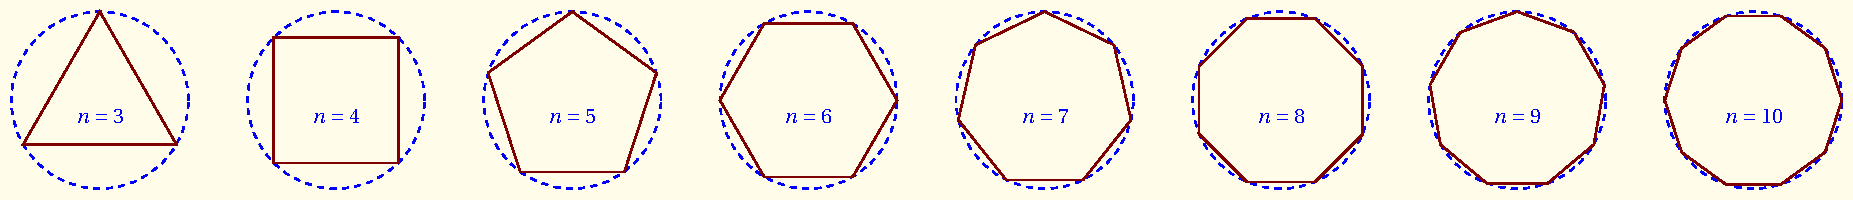
\includegraphics[scale=0.5]{0_home_antalcides_MEGA_calculo_I_libro_pdf_poligonos.pdf}\caption{Polígonos inscritos en una circunferencia}\label{fig:poligono}
\end{figure}

\end{ejemplo}

\begin{defi}{Sucesión acotada superiormente}{acotsup}

Se dice que una sucesión, $a_{n},$ es acotada superiormente, cuando
existe un número real $K$, llamado cota superior de la sucesión,
tal que $a_{n}<K,$ para todo $n$ ( es decir todos los elementos
de la sucesión son menores que $K).$ 

\end{defi}

\begin{ejercicio}[Sucesión acotada superiormente]

Demostrar que la sucesión $\left\{ \dfrac{n}{n+1}\right\} $ es acotada
superiormente.

\end{ejercicio}

\subsection{Sucesión acotada inferiormente.}

\begin{ejemplo}

La sucesión de las áreas de los polígonos regulares circunscritos
en una circunferencia, cuando el número de lados se aumenta indefinidamente,
tiene la propiedad de que todos sus términos son mayores que el área
des circulo correspondiente, en un caso como este se dice que la sucesión
está acotada inferiormente. 

\begin{figure}[H]
\centering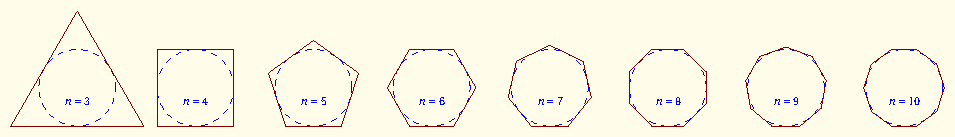
\includegraphics{1_home_antalcides_MEGA_calculo_I_libro_pdf_poligonoreg1.pdf}\caption{Polígonos circunscritos en una circunferencia}\label{fig:poligono2}
\end{figure}

\end{ejemplo}

\begin{defi}{Sucesión acotada superiormente}{acotinf}

Se dice que una sucesión, $a_{n},$ es acotada inferiormente, cuando
existe un número real $M$, llamado cota inferior de la sucesión,
tal que $a_{n}>M,$ para todo $n$ ( es decir todos los elementos
de la sucesión son mayores que $M).$ 

\end{defi}

\begin{ejercicio}[Sucesión acotada superiormente]

Demostrar que la sucesión $\left\{ \dfrac{n+1}{n}\right\} $ es acotada
superiormente.

\end{ejercicio}

\subsection{Sucesión acotada.}

\begin{defi}{Sucesión acotada }{acot}

Se dice que una sucesión, $a_{n},$ es acotada cuando lo es superiormente
e inferiormente, es decir, cuando admite una cota superior $M$ y
una cota inferior $K$ .

Se cumplirá por tanto que existen números reales $M$ y $K$ tal que
$M<a_{n}<K,$ para todo $n.$ 

\end{defi}

\noun{Geométricamente}: La sucesión acotada queda representada si
se encuentra totalmente dentro del segmento $MK.$

\subsection{Sucesión infinita.}

\begin{defi}{Sucesión infinita}{sinf}

Se dice que una sucesión, $a_{n},$ es infinita si no está acotada. 

\end{defi}

Este concepto será más, como un caso especial de límite.

\noun{Geométricamente}: Si una sucesión es infinita, no existe un
segmento, por grande que se considere, que contenga a todos los puntos
de la sucesión. 

\begin{ejemplos}

Las sucesiones siguientes son infinitas, es decir, no acotadas.
\begin{enumerate}
\item $\left\{ n^{2}\right\} $ Esta sucesión no está acotada superiormente,
pues dado un número $K$, por grande que sea, para que $n^{2}>K,$
bastará tomar un $n>\sqrt{K}.$
\item la sucesión $\left\{ \left(-n\right)^{3}\right\} $ no está acotada
inferiormente, pues dado un número, $M,$ por pequeño que sea para
que $\left(-n\right)^{3}<M,$ bastará tomar $n>\sqrt[3]{M}$ (pues
entonces $\left|\left(-n\right)^{3}\right|>M,$ y por tanto $\left(-n\right)^{3}<M,$
recuerde que si un número negativo tiene modulo mayor que otro número,
el primero es menor que el segundo). 
\end{enumerate}
\end{ejemplos}

\subsection{Sucesiones monótonas.}

\begin{defi}{Sucesiones monótonas}{smon}

Una sucesión cuyos términos se suceden siempre creciendo se llama
monótona creciente, ( $a_{i}>a_{j}$ siempre que $i>j$). Una secesión
cuyos términos se suceden decreciendo sin cesar se llama monótona
decreciente ( $a_{1}<a_{j}$ siempre que $i<j$). 

\end{defi}

\begin{ejemplo}

Las aproximaciones decimales sucesivas por defecto de la $\sqrt{2}$
forman una sucesión monótona creciente, y las aproximaciones por exceso
forman una sucesión monótona decreciente.

\end{ejemplo}

\section{Nociones preliminares necesarias para el estudio de límites.}

\intro

A nuestro juicio, la falta de comprensión del concepto de límite,
por parte de la mayoría de los estudiantes, radican en las siguientes
causas 
\begin{enumerate}
\item La falta de un apoyo intuitivo que permita la asimilación de la definición
abstracta (general).
\item La falta de dominio del cálculo con desigualdades (leyes de monotonía), 
\item La falta de un conocimiento claro de las relaciones modulares y de
sus interpretaciones geométricas.
\end{enumerate}
Es muy probable que muchos alumnos no hayan tenido nunca una idea
clara de las leyes de monotonía ni del significado de las desigualdades
en las que figuran módulos; y en el supuesto de que la hayan tenido
, al llegar al 11º grado de bachillerato la han olvidado. siendo así
es muy difícil que entiendan una definición abstracta construida basada
en estos elementos.

Por este motivo repasaremos en esta sección los conceptos instrumentales
necesarios para una buena comprensión del concepto de límite y de
sus propiedades.

\subsection{Reglas de cálculo con desigualdades (leyes de la monotonía).}

\subsubsection{Ley de la suma de desigualdades.}

%\vspace*{10pt}

\begin{propiedad}{}

Sumando miembro a miembro varias desigualdades del mismo sentido,
se obtiene otra desigualdad del mismo sentido.

\end{propiedad}

es decir podemos hacer lo siguiente. 
\[
\begin{array}{ccc}
a & < & b\\
c & < & d\\
\hline a+c & < & b+d
\end{array}\;\;\text{o\;\;\ensuremath{\begin{array}{ccc}
 \text{\text{\ensuremath{a}}}  &  >  &  \text{\ensuremath{b}}\\
 \text{\ensuremath{c}}  &  >  &  \text{\ensuremath{d}}\\
\hline \text{\ensuremath{a+c}}  &  >  &  \text{\ensuremath{b+d}} 
\end{array}}}
\]
\begin{ejemplos}
\begin{enumerate}
\item Si $\left\{ \begin{array}{ccc}
1 & < & 4\\
2 & < & 5\\
4 & < & 7
\end{array}\right.,$ entonces $1+2+4<4+5+7$ por tanto $7<16.$
\item Si $\left\{ \begin{array}{ccc}
-2 & < & 1\\
-4 & < & -3
\end{array}\right.,$ entonces $\left(-2\right)+\left(-4\right)<1+\left(-3\right)$ por
tanto $\left(-6\right)<\left(-2\right).$
\item En general si $\left\{ \begin{array}{ccc}
a_{1} & < & b_{1}\\
a_{2} & < & b_{2}\\
a_{3} & < & b_{3}\\
\vdots & \vdots & \vdots\\
a_{n} & < & b_{n}
\end{array}\right.,$ entonces \foreignlanguage{english}{$\begin{array}{ccc}
a_{1} & < & b_{1}\\
a_{2} & < & b_{2}\\
a_{3} & < & b_{3}\\
\vdots & \vdots & \vdots\\
a_{n} & < & b_{n}\\
\hline a_{1}+a_{2}+a_{3}+\cdots+a_{n} & < & b_{1}+b_{2}+b_{3}+\cdots+b_{n}
\end{array}\;$}
\end{enumerate}
\end{ejemplos}

\begin{ejercicio}[]

Dadas las desigualdades $2<5\;x>y,\;a<b;$ obtener una nueva desigualdad
aplicando la suma de desigualdades (\noun{Sugerencia}: debe colocar
todas las desigualdades con el mismo sentido antes de sumarlas)

\end{ejercicio}

\subsubsection{Leyes de monotonía para la diferencia.}

\vspace*{10pt}

\begin{propiedad}{}

Si a los dos miembros de una desigualdad se les resta un mismo número
se obtiene otra desigualdad del mismo sentido.

\end{propiedad}

\begin{ejemplos}
\begin{enumerate}
\item Si $12<15,$ entonces $12-3<15-3,$ o sea, $9<12.$
\item Si $a>b,$ entonces $a-c>b-c$.
\end{enumerate}
\end{ejemplos}

\begin{propiedad}{}

Si a los dos miembros de una igualdad se les restan los miembros de
una desigualdad, se obtiene otra desigualdad de sentido contrario.

\end{propiedad}

\begin{ejemplos}
\begin{enumerate}
\item Si $3=3$ y $7>5,$ entonces $3-7<3-5,$ o sea, $-4<-2.$
\item En general: Si $a=b$ y $c<d$ entonces $a-c>b-d$.
\end{enumerate}
\end{ejemplos}

\begin{propiedad}{}

Si se restan miembro a miembro dos desigualdades, de sentidos contrarios,
se obtiene otra desigualdad con el sentido de la primera .

\end{propiedad}

\begin{ejemplos}
\begin{enumerate}
\item Si $8>2$ y $4<6,$ entonces $8-4>2-6,$ o sea, $4>-4.$
\item En general: Si $a<b$ y $c>d$ entonces $a-c<b-d$.
\end{enumerate}
\end{ejemplos}

\subsubsection{Leyes de la monotonía para la multiplicación. }

\vspace*{10pt}

\begin{propiedad}{}

Multiplicando miembro a miembro dos desigualdades del mismo sentido
y con términos positivos, se obtiene otra desigualad del mismo sentido
.

\end{propiedad}

es decir si $a,\;b,\;c$ y $d$ son números positivos, podemos hacer
lo siguiente. 
\[
\begin{array}{ccc}
a & < & b\\
c & < & d\\
\hline a\cdot c & < & b\cdot d
\end{array}\;\;\text{o\;\;\ensuremath{\begin{array}{ccc}
 \text{\text{\ensuremath{a}}}  &  >  &  \text{\ensuremath{b}}\\
 \text{\ensuremath{c}}  &  >  &  \text{\ensuremath{d}}\\
\hline \text{\ensuremath{a\cdot c}}  &  >  &  \text{\ensuremath{b\cdot d}} 
\end{array}}}
\]
\begin{ejemplos}
\begin{enumerate}
\item Si $8>2$ y $4>6,$ entonces $8\cdot4>2\cdot6,$ o sea, $32>12.$
\item  Si $2<4$ y $1<5$ entonces $2\cdot1<4\cdot5,$ o sea $2<20$.
\end{enumerate}
\end{ejemplos}

\begin{propiedad}{}

Si multiplicamos los miembros de una desigualdad por un número positivo,
la desigualdad resultante tiene el mismo sentido de la original.

\end{propiedad}

es decir si $a>0$ y, $b>c$ entonces $a\cdot b>a\cdot c$, o si $b<c$
entonces $a\cdot b<a\cdot c$.

\begin{propiedad}{}

Si multiplicamos los miembros de una desigualdad por un número negativo,
la desigualdad resultante cambia de sentido con respecto a la original.

\end{propiedad}

es decir si $a<0$ y, $b>c$ entonces $a\cdot b<a\cdot c$, o si $b<c$
entonces $a\cdot b>a\cdot c$.\begin{ejemplos}
\begin{enumerate}
\item Si $8=8$ y $4<6,$ entonces $8\cdot4<8\cdot6,$ o sea, $32<48.$
\item Si $-2=-2$ y $5>1$ entonces $-2\cdot5<-2\cdot1,$ o sea $-10<-2$.
\end{enumerate}
\end{ejemplos}

\begin{propiedad}{\label{prop:lmep}}

Si elevamos los dos miembros de una desigualdad con términos positivos,
a una potencia positiva, se obtiene una desigualdad del mismo sentido.
Si el exponente es negativo se invierte el sentido de la desigualdad.

\end{propiedad}

es decir si $a,b>0$; $n>0$ y $a>b,$ entonces $a^{n}>b^{n}$, y
$a^{-n}<b^{-n}.$

\begin{ejemplos}
\begin{enumerate}
\item Si $4<6,$ entonces $4^{2}<6^{2},$ o sea, $16<36.$
\item Si $5>1$ entonces $5^{-3}<1^{-3},$ o sea $\frac{1}{125}<1$.
\end{enumerate}
\end{ejemplos}

\obs Cuando el exponente es fraccionario la propiedad \myref{prop:lmep}
podemos aplicarla a la radicación.

\subsubsection{Leyes de la monotonía para la división}

\vspace*{10pt}

\begin{propiedad}{}

Si dividimos miembro a miembro los términos de dos desigualdades con
términos positivos, y con sentidos contrarios, obtenemos una desigualdad
con el sentido del dividendo.

\end{propiedad}

es decir si $a,b,c,d>0$ y, $a>b,\;c<d$ entonces $\frac{a\cdot}{c}>\frac{b}{d}$,
o si $a,b,c,d>0$ y, $a<b,\;c>d$ entonces $\frac{a\cdot}{c}<\frac{b}{d}$.

\begin{ejemplos}
\begin{enumerate}
\item Si $4<6$ y $2>1$ entonces $\frac{4}{2}<\frac{6}{1},$ o sea, $2<6.$
\item Si $5>1$ y $10<20$ entonces $\frac{5}{10}>\frac{1}{20},$ o sea
$\frac{1}{2}>\frac{1}{20}$.
\end{enumerate}
\end{ejemplos}

\begin{propiedad}{}

Si a una desigualdad le dividimos sus miembros por términos positivos,
obtenemos una desigualdad con el mismo sentido ,a

\end{propiedad}

es decir si $a>0$ y, $c>b$ entonces $\frac{c\cdot}{a}>\frac{b}{a}$,
o si $a>0$ y, $c<b$ entonces $\frac{c\cdot}{a}<\frac{b}{a}$.

\begin{ejemplo}

Si $4<6$ entonces $\frac{4}{2}>\frac{6}{2},$ o sea, $2<3.$

\end{ejemplo}

\begin{propiedad}{}

Si tenemos una igualdad de miembros positivos, y una desigualdad,
al dividir la ecuación entre la desigualdad miembro a miembro obtenemos
una desigualdad de sentido contrario a la original.

\end{propiedad}

es decir si $a>0$ y, $c>b$ entonces $\frac{a\cdot}{c}<\frac{a}{b}$,
o si $a>0$ y, $c<b$ entonces $\frac{a\cdot}{c}>\frac{a}{b}$.

\begin{ejemplo}

Si $4<6$ entonces $\frac{2}{4}>\frac{2}{6},$ o sea, $\frac{1}{2}>\frac{1}{3}.$

\end{ejemplo}

\subsection{Relaciones entre módulos.}

\begin{defi}{Módulo o valor absoluto}{dmod}

El módulo o valor absoluto de un número real, $a,$ se representa
por $\left|a\right|$ (se lee módulo de $a$) y se define 
\begin{equation}
\left|a\right|=\left\{ \begin{array}{ccc}
-a & \text{si} & a<0\\
0 & \text{si} & a=0\\
a & \text{si} & a>0
\end{array}\right.\label{eq:modulo}
\end{equation}

\end{defi}

\begin{ejemplos}
\begin{enumerate}
\item $\left|-3\right|=-\left(-3\right)=3$.
\item $\left|0\right|=0.$
\item $\left|3\right|=3.$
\end{enumerate}
\end{ejemplos}

De acuerdo con las reglas del cálculo con números reales, recordamos
que se cumplen las siguientes relaciones:

\begin{propiedad}{\hspace{-2pt}:\ Propiedad triangular}

El módulo de una suma de números reales es igual o menor que la suma
de los módulos de los sumandos. resulta igual a la suma de los módulos
cuando todos los sumandos son del mismo signo.

\end{propiedad}

\begin{ejemplos}
\begin{enumerate}
\item $\left|5-2+3-4+1\right|<\left|5\right|+\left|-2\right|+\left|3\right|+\left|-4\right|+\left|1\right|$
entonces $3<15.$
\item $\left|-2-5-7\right|=\left|-2\right|+\left|-5\right|+\left|-7\right|$
entonces $-\left(-14\right)=\left|-14\right|=2+5+7=14.$
\item $\left|3+6\right|=\left|3\right|+\left|6\right|=9.$
\end{enumerate}
\end{ejemplos}

\begin{propiedad}{}

El módulo de un producto es igual al producto de los módulos. 

\end{propiedad}

Es decir $\left|a\cdot b\right|=\left|a\right|\cdot\left|b\right|.$

\begin{ejemplos}
\begin{enumerate}
\item $\left|-3\cdot2\right|=\left|-3\right|\cdot\left|2\right|=6.$
\item $\left|\left(-2\right)\cdot\left(-5\right)\right|=\left|-2\right|\cdot\left|-5\right|=2\cdot5=10.$
\end{enumerate}
\end{ejemplos}

\begin{propiedad}{}

El módulo de un cociente es igual al cociente de los módulos.

\end{propiedad}

Es decir, $\left|\dfrac{a}{b}\right|=\dfrac{\left|a\right|}{\left|b\right|},\;b\neq0.$ 

\begin{ejemplos}
\begin{enumerate}
\item $\left|\dfrac{-2}{5}\right|=\dfrac{\left|-2\right|}{\left|5\right|}=\dfrac{2}{5}.$
\item $\left|\dfrac{-3}{-2}\right|=\dfrac{\left|-3\right|}{\left|-2\right|}=\dfrac{3}{2}.$
\end{enumerate}
\end{ejemplos}

\begin{propiedad}{}

El módulo de una potencia es igual a la potencia del módulo. 

\end{propiedad}

Es decir $\left|a^{n}\right|=\left|a\right|^{n}.$

\begin{ejemplo}

$\left|\left(\dfrac{-2}{5}\right)^{3}\right|=\left|\dfrac{-2}{5}\right|^{3}=\dfrac{8}{125}.$

\end{ejemplo}

\begin{propiedad}{}

El módulo de una raíz es igual a la raíz del mismo índice del módulo
del radicando. 

\end{propiedad}

es decir $\left|\sqrt[n]{a}\right|=\sqrt[n]{\left|a\right|}$.

\begin{ejemplo}

$\left|\sqrt[3]{-8}\right|=\sqrt[3]{\left|-8\right|}=\sqrt[3]{8}=2.$

\end{ejemplo}

\subsection{Interpretación geométrica de algunas relaciones modulares.\label{subsec:Interpretaci=0000F3n-geom=0000E9trica-de}}

\subsubsection{Ecuaciones con módulos.}

\begin{ejemplo}

Resolver la ecuación $\val{x}=3.$ 

\end{ejemplo}

\sol La ecuación $\val{x}=3$ la verifican dos valores $x=-3$ y
$x=3$, cuyas imágenes geométricas son dos puntos simétricos respecto
al origen, situados a una distancia de 3 unidades de dicho origen,
como muestra la figura(\ref{fig:cal_lim1})\fin .
\begin{figure}[H]

\centering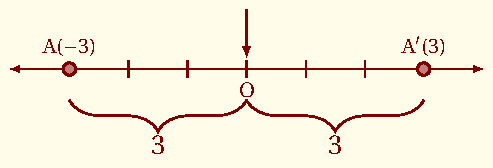
\includegraphics{2_home_antalcides_MEGA_calculo_I_libro_pdf_cal_lim1.pdf}\caption{$\val{x}=3$}\label{fig:cal_lim1}

\end{figure}
\fin

\general La ecuación $\val{x}=K$ tiene como soluciones a $x=-K$
y $x=K,$ cuyas imágenes geométricas son dos puntos simétricos respecto
al origen, situados a $K$ unidades de éste.

\begin{ejemplo}

Resolver la ecuación $\val{x-2}=3.$ 

\end{ejemplo}

\sol La ecuación $\val{x-2}=3$ es verificada por los números que
difieren del 2 en tres unidades, en módulo, ( es decir tres unidades
por debajo y tres unidades por encima se 2); estos números son $x=2-3=-1$
y $x=2+3=5.$

Las imágenes geométricas de estos números son dos puntos simétricos
del punto correspondiente al número 2 y a una distancia de 3 unidades
de él, como se muestra en la figura(\ref{fig:cal_lim2}) 

\begin{figure}[H]
\centering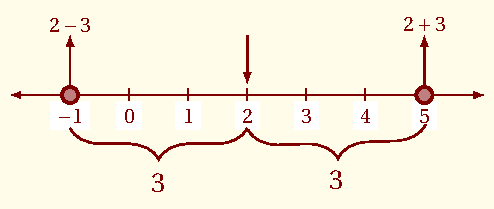
\includegraphics{3_home_antalcides_MEGA_calculo_I_libro_pdf_cal_lim2.pdf}\caption{$\val{x-2}=3$}\label{fig:cal_lim2}
\end{figure}
\fin

\general $\val{x-a}=k$ tiene como soluciones $x=a-k$ y $x=a+k,$
cuyas imágenes geométricas son dos puntos simétricos del punto de
abscisa $a$ y situados a $k$ unidades de él.\vspace*{10pt}

\begin{ejercicios}[]

Resolver las ecuaciones y representar geométricamente sus soluciones.
\begin{enumerate}
\item $\val{x-1}=2,$
\item $\val{x+2}=1,$
\item $\val{x-4}=3.$
\end{enumerate}
\end{ejercicios}

\subsubsection{Inecuaciones con módulos\label{subsec:Inecuaciones-con-m=0000F3dulos}}

\begin{ejemplo}

Resolver la inecuación $\val{x}<5$. 

\end{ejemplo}

\sol La inecuación $\val{x}<5$ la cumplen todos los puntos que distan
del origen menos de 5 unidades, o sea, todos los puntos en el interior
del segmento rectilíneo $AB$, siendo $A\left(-5\right)$ y $B\left(5\right)$
como se observa en la figura(\ref{fig:cal_lim3}). 

\begin{figure}[H]
\centering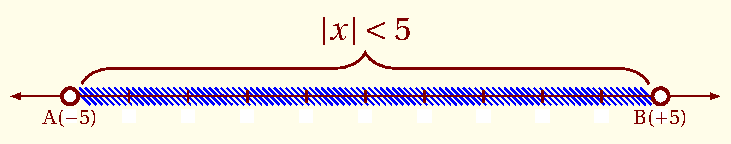
\includegraphics{4_home_antalcides_MEGA_calculo_I_libro_pdf_cal_lim3.pdf}\caption{$\val{x}<5$}\label{fig:cal_lim3}
\end{figure}
\fin

\general $\val{x}<k$ representa a todos los puntos en el interior
que tiene extremos en $A\left(-k\right)$ y $B\left(k\right)$ 

\begin{apunte} \obs

Cuando se considera la relación modular $\val{x}\leq k$ (en vez de
$\ensuremath{\val{x}<5}$), los extremos del segmento $A\left(-k\right)$
y $B\left(k\right),$ quedan incluidos como soluciones de la inecuación,
y se dice que $\ensuremath{\val{x}\leq5}$ representa el segmento
cerrado o completo, mientras que $\ensuremath{\val{x}<5}$representa
el segmento abierto, es decir no contiene los extremos, como se indica
en la figura \ref{fig:cal_lim3a} 

\begin{figure}[H]
\centering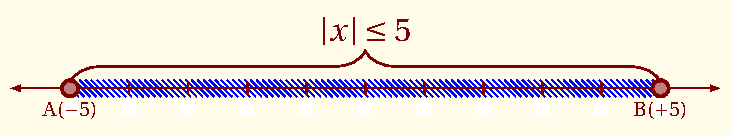
\includegraphics{5_home_antalcides_MEGA_calculo_I_libro_pdf_cal_lim3a.pdf}\caption{$\val{x}\leq 5$}\label{fig:cal_lim3a}
\end{figure}
\fin

\end{apunte}

\begin{ejercicios}[]

Resolver las siguientes Inecuaciones.
\begin{enumerate}
\item $\val{x}\leq3,$
\item $\val{x}<1,$
\item $\val{x}\leq\frac{3}{2}.$
\end{enumerate}
\end{ejercicios}

\paragraph{Entorno de un punto.}

\begin{defi}{Entorno de un punto}{epto}

Llamaremos entorno de un punto a cualquier segmento abierto que contenga
a dicho punto como centro. En particular, un entorno del origen es
cualquier segmento abierto que tenga su punto medio como el origen. 

\end{defi}

Un entorno queda determinado mediante su centro y su amplitud. De
acuerdo con lo tratado en el apartado \ref{subsec:Inecuaciones-con-m=0000F3dulos},
los entornos del origen quedan representados analíticamente mediante
una relación del tipo $\val{x}<k$ (entorno del origen de semi-amplitud
$k)$. en general un entorno de un punto es cualquier segmento abierto
al cual pertenezca el punto, pero nosotros sólo usaremos entornos
simétricos por comodidad.

\begin{ejemplos}\label{ej:ejem1}
\begin{enumerate}
\item El segmento del origen de semi-amplitud 0,001 se representa analíticamente
así: $\val{x}<0.001$, osea el intervalo $\left(-0.0010,0.001\right)$.
\item El entorno del origen de semi-amplitud 1 queda representado por la
inecuación $\val{x}<1.$
\item \begin{flushleft}
\label{itm:ej27}Expresar analíticamente que todos los términos de
la sucesión $\left\{ \dfrac{1}{n}\right\} $ siguientes al término
de lugar 100, pertenecen al entorno de origen de semi-amplitud 0.01.\linebreak{}
\sol Bastará con escribir: $\val{\dfrac{1}{n}}<0.01,$ para todo
$n>100.$ \fin
\par\end{flushleft}
\item Investigar si todos los términos de la sucesión $\left\{ \dfrac{1}{n^{2}}\right\} ,$
a partir de $1$, pertenecen al entorno de origen $\val{x}<0.0001,\inline\text{\label{eq:ec10}},$
e indicar el lugar a partir del cual se cumple la ecuación(\foreignlanguage{english}{\ref{eq:ec10}})
\linebreak{}
\sol De acuerdo con el enunciado deberá cumplirse que: $\val{\dfrac{1}{n^{2}}}<0.0001,$
que por ser $n^{2}$ positivo se puede escribir así; $\dfrac{1}{n^{2}}<0.0001,$
extrayendo la raíz cuadrada en ambos términos obtenemos la desigualdad
$\dfrac{1}{n}<0.01$ ahora multiplicando los dos miembros por $100n$
se obtiene $100<n,$ por tanto, los términos de la sucesión $\left\{ \dfrac{1}{n^{2}}\right\} $
están en el interior del entorno $\val{x}<0.0001,$ para todo $n>100.$
\fin
\item \begin{flushleft}
Dada la sucesión $\dfrac{1}{n+10}$ y el entorno del origen $\val{x}<10^{-12}.$
Investigar si toda la sucesión a partir de un término dado, pertenece
a dicho entorno.\linebreak{}
\sol Deberá cumplirse $\val{\dfrac{1}{n+10}}<10^{-12},$ o lo que
es equivalente, $\dfrac{1}{n+10}<\dfrac{1}{10^{12}},$ (por ser $\dfrac{1}{n+10}$
positivo), podemos multiplicar los dos miembros por $10^{12}\cdot(n+10),$
queda $n+10>10^{12},$ de donde $n>10^{12}-10$.\linebreak{}
\vspace*{2pt}\begin{nota}\peque Observe: cómo se aplican las leyes
de la monotonía o reglas del cálculo con desigualdades en cada una
de las transformaciones que se efectúan hasta lograr que la $n$ quede
despejada en un miembro de la desigualad. \end{nota}Respuesta: Para
tono $n>10^{12}-10$ los términos de la sucesión están en el interior
del entorno dado.\fin
\par\end{flushleft}

\end{enumerate}
\end{ejemplos}

\begin{ejercicios}[]
\begin{enumerate}
\item Representar analíticamente el entorno de origen de semi-amplitud $10^{-6},$
\item Investigar si todos los términos de la sucesión $\left\{ \dfrac{1}{n^{2}}\right\} ,$
siguientes a un cierto término , pertenecen al entorno de origen $\val{x}<10^{-2},\inline\text{\label{eq:ec11}},$
e indicar a partir de que término de la sucesión se cumple la ecuación
\ref{eq:ec11}. 
\item Dada la sucesión $\left\{ \dfrac{2}{n^{2}+1}\right\} $y el entorno
del origen $\val{x}<10^{-6},$ investigue si todos los términos de
la sucesión, a partir de uno, están en el entorno e indicar el valor
de $n$ a partir del cual los términos de la sucesión están en el
interior del entorno dado. 
\item Dada la sucesión $\left\{ \dfrac{n}{n+1}\right\} $y el entorno del
origen $\val{x}<0.99,$ investigue cuantos términos están en el interior
y cuantos están en el exterior del entorno dado.
\end{enumerate}
\end{ejercicios}

\begin{ejemplo}

Resolver la inecuación $\val{x}>3.$ 

\end{ejemplo}

\sol La ecuación $\val{x}>3$ la cumplen todos los puntos que distan
del origen más de tres unidades, geométricamente dichos puntos forman
el exterior del segmento con extremos $A\left(-3\right)$ y $B\left(3\right)$,
como muestra la figura\ref{fig:cal_lim4} 
\begin{figure}[H]
\centering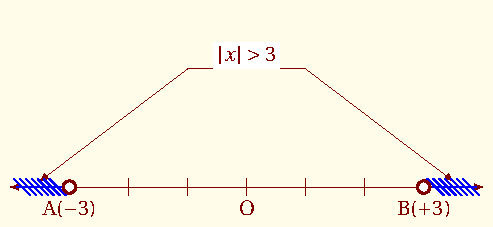
\includegraphics{6_home_antalcides_MEGA_calculo_I_libro_pdf_cal_lim4.pdf}\caption{$\val{x}> 3$}\label{fig:cal_lim4}
\end{figure}
\fin

\general La inecuación $\val{x}>k$ representa el exterior del segmento
con extremos $A\left(-k\right)$ y $B\left(k\right).$ 

\begin{ejercicios}[] Señalar sobre una recta metrizada las regiones
representadas por las siguientes relaciones modulares:
\begin{enumerate}
\item $\val{x}>2,$
\item $\val{x}\leq5,$
\item $\val{x}\geq3,$
\item $\val{x}\geq\frac{3}{4},$
\item $\val{x}\leq\frac{1}{2}$
\end{enumerate}
\end{ejercicios}

\begin{ejemplo}\label{ej:ejem5cv}

Resolver la inecuación $\val{x-2}<3.$

\end{ejemplo}

\sol La inecuación $\val{x-2}<3$ la verifican todos los números
que difieren del $2$, en módulo, menos de tres unidades. La imagen
geométrica de dicha inecuación es el interior del segmento con centro
$2$ y semi-amplitud tres unidades, pero este segmento es el entorno
del punto $2$ con semi-amplitud $3,$como muestra la figura \ref{fig:cal_lim5}
\begin{figure}[H]
\centering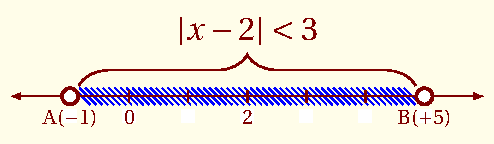
\includegraphics{7_home_antalcides_MEGA_calculo_I_libro_pdf_cal_lim5.pdf}\caption{$\val{x-2}< 3$}\label{fig:cal_lim5}
\end{figure}
\fin

\general La inecuación $\val{x-a}<k$ la verifican todos los números
que son mayores de $a-k$ y menores de $a+k$, o sea, todos los números
$x$ que cumplen: $a-k<x<a+k.$ \noun{Geométricamente:} Dichos puntos
forman el interior del segmento $AB,$ siendo $A\left(a-k\right),$
$B\left(a+k\right)$, o sea: El entorno del punto $a$ de semi-amplitud
$k.$

\begin{nota}\peque

Es muy importante, para una buena comprensión del concepto fundamental
de límite, que el lector maneje con mucha habilidad las relaciones
modulares de este tipo, así como sus interpretaciones geométricas. 

\end{nota}

\begin{ejemplos}
\begin{enumerate}
\item La inecuación $\val{x-5}<6$ representa al entorno del punto $P\left(5\right)$de
semi-amplitud $6$ unidades. Los extremos $A$ y $B$ de este entorno
son: 
\[
A\left(5-6\right)\equiv A\left(-1\right)\text{ y \ensuremath{B\left(5+6\right)\equiv B\left(11\right).}}
\]
\item La inecuación $\val{x+1}<2$ representa el entorno del punto $Q\left(-1\right)$de
semi-amplitud $2$ unidades. (Note que $\val{x+1}=\val{x-\left(-1\right)}$).
\item Investigar el término de la sucesión $\left\{ \dfrac{n}{n+1}\right\} $están
en el interior del entorno del punto $1$ y semi-amplitud $0.01$a
partir de un valor de $n.$ \linebreak{}
\sol Los puntos de la sucesión que verifican la inecuación $\val{x-1}<0.01$
cumplirán que $\val{\dfrac{n}{n+1}-1}<0.01,$ o sea, $\val{\dfrac{n-n-1}{n+1}}<\dfrac{1}{100},$
o bien $\dfrac{1}{n+1}<\dfrac{1}{100},$ ahora si multiplicamos ambos
miembros de la inecuación por $100\left(n+1\right),$ obtenemos $100<n+1,$
de donde $n>99.$ \linebreak{}
\resp Los puntos de la sucesión $\left\{ \dfrac{n}{n+1}\right\} $que
se encuentran en el interior del punto $1$, $\val{x-1}<0.01$, son
todos los que cumplen que $n>99.$\fin
\end{enumerate}
\end{ejemplos}

\begin{ejercicios}[]
\begin{enumerate}
\item Descubrir los números los números que satisfacen a las siguientes
inecuaciones y dibujar los segmentos correspondientes en una recta
metrizada.
\begin{enumerate}
\item $\val{x-1}<3,$
\item $\val{x+3}<2,$
\item $\val{x-\frac{1}{2}}<\frac{2}{3},$
\item $\val{x+4}<\frac{1}{4},$
\item $\val{x+4}<2,$
\item $\val{x+\alpha}<\epsilon,$
\end{enumerate}
\item Investigue cuantos términos de la sucesión $\left\{ \dfrac{2n-1}{n+2}\right\} $
pertenecen al entorno $\val{x-2}<0.0001,$ y cuantos no pertenecen.
\end{enumerate}
\end{ejercicios}

\begin{ejemplo}

Resolver la inecuación $\val{x-1}>2$

\end{ejemplo}

\sol La inecuación $\val{x-1}>2,$ la cumplen todos los números que
difieren de $1,$ en módulo, más de dos unidades, osea, todos los
números que son menores de $1-2=-1$ y mayores de $1+2=3.$

\noun{Geométricamente}: Dichos números corresponden a los puntos exteriores
del segmento formado por los extremos $A\left(-1\right)$ y $B\left(3\right),$
como se muestra en la figura(\ref{fig:cal_lim6})
\begin{figure}[H]
\centering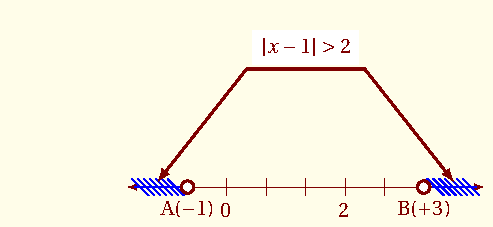
\includegraphics{8_home_antalcides_MEGA_calculo_I_libro_pdf_cal_lim6.pdf}\caption{$\val{x-1}>2$}\label{fig:cal_lim6}
\end{figure}
\fin

\general La inecuación $\val{x-a}>k,$ la cumplen todos los números
que son menores que $a-k,$ y mayores que $a+k,$ o sea, todos los
números que cumplen: $x<a-k$ y .

\emph{\noun{Geométricamente}}: Los puntos correspondientes a los números
que verifican $\val{x-a}>k$ forman el exterior del segmento con extremos
$A\left(a-k\right)$ y $B\left(a+k\right).$

\begin{ejercicios}[]

Descubrir los números que satisfacen las inecuaciones dadas y representarlas
en una recta metrizada.
\begin{enumerate}
\item $\val{x-2}>4,$ 
\item $\val{x+3}>5,$
\item $\val{x-3}>3,$
\item $\val{x+\frac{1}{2}}>4.$ 
\end{enumerate}
\end{ejercicios}

\section{El concepto fundamental de sucesión infinitésima.}

\intro 

Damos a continuación una explicación detallada, mediante ejemplos,
del concepto de infinitésimo. Después de estudiar cuidadosamente los
ejemplos el lector queda preparado para comprender bien la definición
general, que fijará definitivamente mediante la resolución de ejercicios.

\begin{ejemplo}\label{ej:ejem2.1}

En el ítem \ref{itm:ej27} del ejemplo(\myref{ej:ejem1}) vimos que
los términos de la sucesión $\left\{ \dfrac{1}{n}\right\} $ son menores
que $0.01$ para todo $n>100.$ Análogamente, si en vez de fijar el
valor $0.01$ fijamos otro más pequeño, por ejemplo, $0.0001,$ se
cumplirá que $\val{\dfrac{1}{n}}<0.0001$ para todo $n>10000;$ pero
si queremos demostrar que, por pequeño que se fije un número los términos
de $\left\{ \dfrac{1}{n}\right\} $ quedan menores que él, a partir
de un término, tendremos que recurrir a la notación literal; Representemos
con la letra $\epsilon$ (epsilon), a cualquier numero positivo; si
logramos probar que $\val{\dfrac{1}{n}}<\epsilon,$ para todo $n$
superior a un cierto valor, como $\epsilon$ representa a cualquier
número positivo, quedará demostrado que la sucesión $\left\{ \dfrac{1}{n}\right\} $
tiene la propiedad de que sus términos son, en módulo, menores que
cualquier número positivo, a partir de uno de ellos. Pero en efecto:
para que $\val{\dfrac{1}{n}}<\epsilon,$ o sea, $\dfrac{1}{n}<\epsilon$
basta con que $n>\dfrac{1}{\epsilon}.$\linebreak{}
\end{ejemplo}

\conclu Dado un número positivo cualquiera $\epsilon,$ en particular
tan pequeño como queramos, los términos de la sucesión$\left\{ \dfrac{1}{n}\right\} $
tienen la propiedad de ser en módulo menores que $\epsilon$ para
todo $n<\dfrac{1}{\epsilon}.$ Las sucesiones que cumplen esta propiedad
se llaman sucesiones infinitésimas.

\noun{Interpretación geométrica}: Decir que $\dfrac{1}{n}<\epsilon$
para todo $n>\dfrac{1}{\epsilon},$ equivale a decir que los términos
de la sucesión $\left\{ \dfrac{1}{n}\right\} $ que pertenecen al
entorno del origen de semi-amplitud $\epsilon$ para todo $n>\dfrac{1}{\epsilon},$
o sea, desde un término en adelante. En otras palabras: Rodeado el
origen de un entorno cualquiera, en particular tan pequeño como queramos,
todos los términos de la sucesión, a partir de uno, sin excepción,
están en dicho entorno; por tanto: fuera del entorno del origen hay
un número finito de términos de la sucesión y en el interior un número
infinito. Tenemos caracterizada así una sucesión infinitésima por
la siguiente propiedad geométrica: Cualquier entorno del origen, por
pequeño que sea, contiene infinitos puntos de la sucesión. La expresión
analítica de esta propiedad, definidora de las sucesiones infinitésimas,
es la siguiente: 

La inecuación $\val{x}>\epsilon$ solo la cumplen un número finito
de términos de $\{a_{n}\}$; por tanto, la inecuación $\val{x}<\epsilon$
la verifican un número infinito de términos de $\{a_{n}\},$ donde
$\epsilon$ representa a cualquier número positivo, en particular
tan pequeño como queramos. 

\begin{ejemplo}\label{ej:lim33}

\begin{wrapfigure}{r}{0.4\linewidth} \centering

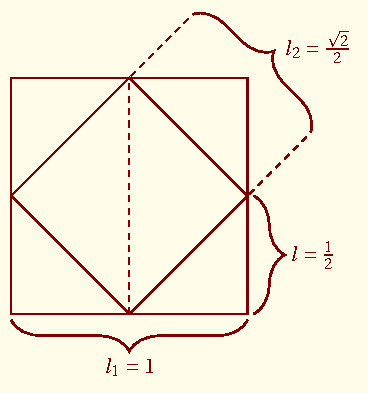
\includegraphics{9_home_antalcides_MEGA_calculo_I_libro_pdf_cal_lim7.pdf}
\caption{Sucesi\'on de cuadrados}
\label{fig:cal_lim7} \end{wrapfigure}

Consideremos un cuadrado de lado unidad que representaremos por $C_{1}.$
Si se unen los puntos medios de sus lados (los puntos medios de los
lados del cuadrado son extremos de segmentos rectilíneos), se obtiene
otro cuadrado, $C_{2};$ uniendo los puntos medios de los lados de
$C_{2}$ se obtiene un cuadrado $C_{3}$, y continuando así indefinidamente
, uniendo cada vez los puntos medios de los lados del último cuadrado
obtenido, se llega a una sucesión de cuadrados: $C_{1},\;C_{2},\;C_{3},\cdots,\;C_{n},\cdots$.

Representaremos las áreas de estos cuadrados por

$S_{1},\:S_{2}\;S_{3},\cdots,\;S_{n},\cdots,$ respectivamente.

En primer lugar calculemos la expresión del área $S_{n}$ .

$S_{1}=1$, $S_{2}=\left(\dfrac{\sqrt{2}}{2}\right)^{2}=\dfrac{1}{2},$
pues los cuatro triángulos rectángulos isósceles de las esquinas de
$C_{1}$ son congruentes a los cuatros triángulos en los que se descompones
el cuadrado interior $C_{2};$ por tanto $S_{n-1}=\dfrac{1}{2}S_{n}$,
es decir para obtener el área del cuadrado interno se multiplica por
$\dfrac{1}{2}$ el área del cuadrado externo. de esta forma la sucesión
de las áreas sería
\[
1,\dfrac{1}{2},\dfrac{1}{4},\dfrac{1}{2},\cdots,\dfrac{1}{2^{n-1}},\cdots,
\]
es decir la sucesión se representaría como $\left\{ \dfrac{1}{2^{n-1}}\right\} .$ 

Es fácil deducir, por intuición, que el área $S_{n}$ puede llegar
a ser tan pequeña como queramos, tomando $n$ lo suficientemente grande,
pero esto debe ser demostrado matemáticamente, es decir, debemos probar
que dado $\epsilon>0$ cualquiera, se puede encontrar un término de
$\left\{ \dfrac{1}{2^{n-1}}\right\} $ tal que él y todos los siguientes
son menores en modulo que $\epsilon.$

En efecto: Para que $\val{\dfrac{1}{2^{n-1}}}<\epsilon,$ o lo que
es lo mismo, para que $\dfrac{1}{2^{n-1}}<\epsilon,$ basta con que
sea $2^{n-1}>\epsilon,$ o sea: 

$\left(n-1\right)\ln2>\ln\left(\dfrac{1}{\epsilon}\right),$ o bien,
$n-1>\dfrac{\ln\left(\frac{1}{\epsilon}\right)}{\ln2},$ de donde
$n>1+\dfrac{\text{\ensuremath{\ln\left(\frac{1}{\epsilon}\right)}}}{\ln2}.$

\conclu La sucesión $\left\{ \dfrac{1}{2^{n-1}}\right\} $ es infinitésima,
pues dado un $\epsilon>0,$ cualquiera se tiene que $\val{\dfrac{1}{2^{n-1}}}<\epsilon$
para todo $n>1+\dfrac{\text{\ensuremath{\ln\left(\frac{1}{\epsilon}\right)}}}{\ln2}.$

\end{ejemplo}

\begin{defi}{Sucesión infinitésima}{suc-inf}\label{def:suc-inf}

Se dice $\left\{ a_{n}\right\} $ es una sucesión infinitésima cuando
cumple la siguiente propiedad:

Fijando un número positivo cualquiera , $\epsilon>0,$ (en particular
tan pequeño como queramos), todos lo términos de la sucesión a partir
de uno, son menores en módulo que $\epsilon.$ 

\end{defi}

Podemos expresar la anterior definición como: Una sucesión $\left\{ a_{n}\right\} $
se llama infinitésima si para todo $\epsilon>0,$ $\abs{a_{n}}<\epsilon$
desde un $a_{n}$ en adelante.

\noun{Interpretación Geométrica}: La sucesión $\left\{ a_{n}\right\} $
es infinitésima si, rodeado del origen de un entorno cualquiera, (en
particular tan pequeño como queramos), todos los términos de la sucesión,
a partir de uno, están en el interior de dicho entorno.

Por tanto: Cualquier entorno del origen, por pequeño que sea, contiene
infinitos términos de la sucesión (todos a partir de uno) y fuera
de dicho entorno sólo habrá un número finito de términos de la sucesión. 

\notacion Para Indicar que $\left\{ a_{n}\right\} $ es infinitésima
escribiremos: $\left\{ a_{n}\right\} \rightarrow0,$ que se lee la
sucesión $\left\{ a_{n}\right\} $ \textbf{\textsl{tiende a cero}}.

Cuando una sucesión es infinitésima se dice también que tiene límite
cero, y se escribe:
\[
\lim_{n\rightarrow\infty}a_{n}=0
\]

que se lee: \textbf{\textsl{el límite de $a_{n}$ es igual a cero
cuando $n$ tiende a infinito}} ($\infty).$

\begin{ejercicios}[]
\begin{enumerate}
\item Probar que la sucesión $\left\{ \dfrac{1}{n^{2}+1}\right\} $ es infinitésima.
( hay que demostrar que, cualquiera que sea $\epsilon>0,$ $\val{\dfrac{1}{n^{2}+1}}<\epsilon$
para todos los términos siguientes a uno dado).
\item Demostrar que la sucesión de perímetros de los cuadrados $C_{1},\;C_{2},\;C_{3},\cdots,\;C_{n},\cdots$,
del ejemplo \myref{ej:lim33} es una sucesión infinitésima. ( \noun{Indicación}:
El término n-ésimo de la sucesión es: $\dfrac{4}{2\frac{n-1}{2}},$
y se tiene que probar que $\val{\dfrac{4}{2\frac{n-1}{2}}}<\epsilon$
para todo $n>1+\dfrac{2}{\ln2}\ln\left(\frac{4}{\epsilon}\right)$).
\item Demostrar que $\left\{ \sen a_{n}\right\} $es infinitésima, siendo
$\left\{ a_{n}\right\} $ infinitésima (Indicación: basta tener en
cuenta que $\sen a_{n}<a_{n}$).
\item Demostrar que $\left\{ \val{\dfrac{1}{n^{3}-9}}\right\} $ es infinitésima.
\item Dar la interpretación geométrica cartesiana de una sucesión infinitésima.
\end{enumerate}
\end{ejercicios}

\section{El concepto fundamental de límite de una sucesión.}

\intro

En está sección explicaremos el concepto de límite, haciéndolo depender
del concepto de infinitésimo.

Así procederemos también con las reglas del cálculo de límites, es
decir, que las haremos depender del cálculo con infinitésimas. este
no es el camino más directo, pero lo hace más fácil de entender. Después
de un estudio detallado del concepto de límite mediante a través del
concepto de infinitésimos, lo enunciaremos en las diferentes formas
que son usuales en los cursos de Análisis matemático.

Como lo que perseguimos fundamentalmente, más que dar expresiones
muy concisas, lo cual sería más rápido, es que el lector comprenda
lo mejor posible este importante concepto, daremos ejemplos que sirven
de base para construir la definición general y después propondremos
ejercicios que permitan al lector construir ideas que lo lleven a
comprender la definición como síntesis propia. 

\begin{ejemplo}\label{ej:ejem2.3}

Consideremos la sucesión $\left\{ \dfrac{n+1}{n}\right\} .$ Al desarrollarla
obtenemos $\frac{2}{1},\;\frac{3}{2},\;\frac{4}{3},\;\cdots,\;\left(1+\frac{1}{n}\right),\cdots.\inline\text{\label{eq:ec2.4}}$ 

Si observamos los términos de la ecuación \ref{eq:ec2.4} vemos que
se va acercando más y más al valor de $1$, pero esta afirmación debe
ser precisada matemáticamente, lo cual se consigue con facilidad por
medio del concepto de infinitésima, que ya fue definido en \myref{def:suc-inf}.
En efecto, si la sucesión de la ecuación \ref{eq:ec2.4} tiende a
$1,$ al restarle una unidad a tos sus términos, la sucesión resultante
debe tender a cero, o sea debe ser infinitésima; pero el resultado
de restar una unidad a todos los términos de la sucesión de la ecuación
\ref{eq:ec2.4} es la siguiente sucesión: $1,\;\frac{1}{2},\;\frac{1}{3},\;\cdots,\;\frac{1}{n},\cdots,$
que efectivamente es infinitésima (recuerde el ejemplo \myref{ej:ejem2.1}
). 

\end{ejemplo}

\resu Decir que la sucesión $\left\{ \dfrac{n+1}{n}\right\} $ tiende
a $1,$ o tiene límite $1,$ lo cual se indica así: $\left\{ \dfrac{n+1}{n}\right\} \rightarrow1$
ó bien \Lim{\dfrac{n+1}{n}}{n}{\infty}=1,  significa que $\left\{ \dfrac{n+1}{n}-1\right\} =\left\{ \dfrac{1}{n}\right\} $
es una sucesión infinitésima; como esto es cierto, también los es
que el límite de $\left\{ \dfrac{n+1}{n}\right\} $ es igual a $1.$

\begin{ejemplo}

Consideremos un vaso de volumen $V$ e imaginemos las siguientes operaciones:
llenar la mitad del vaso, después agregar la mitad de lo que queda
por llenar y continuar así indefinidamente agregando cada vez la mitad
de agua que falta para llenarse. 

\end{ejemplo}

\sol Se comprende fácilmente que, por este procedimiento, nunca lograríamos
llenar por completo el vaso, pues cada vez se agrega la mitad de lo
que falta para llenarse; pero también se comprende fácilmente que
las cantidades de aguas sucesivas contenidas por el vaso forman una
sucesión que tiende al volumen del vaso, o que tiene por límite el
volumen del vaso. pero un matemático no puede conformarse con una
idea intuitiva, sino que tiene que precisarla aritméticamente, (esto
fué lo que hicieron Cauchy y Weierstrass en el siglo XIX). De acuerdo
con lo dicho en el ejemplo \myref{ej:ejem2.3}, la frase: <<\textbf{El
límite de la sucesión de los volúmenes de agua contenidos sucesivamente
por el vaso es igual al volumen $V$, del vaso}>> es equivalente\footnote{Recordamos que, según se estudia en lógica, dos enunciados son equivalentes,
cuando los dos son verdaderos o falsos al mismo tiempo, es decir,
no puede darse el caso de que uno se verdadero y el otro falso. Cuando
dos enunciados son equivalentes se dice Matemáticas que el uno es
condición necesaria y suficiente para el otro.}a esta otra <<\textbf{al restar a la sucesión de volúmenes de agua
que va conteniendo el vaso la cantidad $V,$ se obtiene una sucesión
infinitésima}>>, cuya veracidad puede ser comprobada aritméticamente.

Para ello, antes de nada, obtengamos la sucesión de volúmenes de agua
que va conteniendo el vaso: El volumen de agua después de la primera
operación será $V_{1}=\left(V-\dfrac{V}{2}\right)$; el volumen después
dela segunda operación es; $V_{2}=\left(V-\dfrac{V}{2^{2}}\right),$
esto es después de la segunda operación solo le falta al vaso para
llenarse $\dfrac{V}{4}=\dfrac{V}{2^{2}}.$ Por un razonamiento análogo,
el volumen contenido por el vaso después de la tercera operación será;
$V_{3}=\left(V-\dfrac{V}{2^{3}}\right),$ y así sucesivamente, el
volumen contenido después de $n$ operaciones será; $V_{n}=\left(V-\dfrac{V}{2^{n}}\right)$
por tan to la sucesión de los volúmenes de agua contenida sucesivamente
por el vaso tiene por tanto la siguiente expresión general: $\left\{ V-\dfrac{V}{2^{n}}\right\} ,\inline\text{\label{eq:ec2.5}}$

Si a todos los términos de está sucesión le restamos la cantidad $V$
nos que la siguiente sucesión: $\left\{ -\dfrac{V}{2^{n}}\right\} .$

Si logramos probar que esta última sucesión es infinitésima, quedará
demostrada la ecuación \ref{eq:ec2.5} tiende a $V$.

Ahora bien, probar que $\left\{ -\dfrac{V}{2^{n}}\right\} \inline\text{\label{eq:ec2.6}},$
es infinitésima, es equivalente a probar que, dado un $\epsilon>0$
o cualquiera, todos los términos de la ecuación \ref{eq:ec2.6} a
partir de uno, son en módulo menores que $\epsilon,$ o sea, que hay
que probar que $\val{\dfrac{-V}{2^{n}}}=\dfrac{V}{2^{n}}<\epsilon,\text{\inline\text{\label{eq:ec2.7}},}$
a partir de un valor de $n.$ Pero la ecuación \ref{eq:ec2.7} se
cumple siempre que $2^{n}>\frac{V}{\epsilon}$ o sea, siempre que
$n\ln2>\ln\left(\frac{V}{\epsilon}\right),$ de donde 
\[
n>\dfrac{\ln\left(\frac{V}{\epsilon}\right)}{\ln2}.
\]
Al haber probado que la sucesión $\left\{ \left(V-\dfrac{V}{2^{n}}\right)-V\right\} $
es infinitésima, ha quedado demostrado que el límite de $\left\{ V-\dfrac{V}{2^{n}}\right\} $
es igual a $V$. \fin

Más adelante cuando se expliquen las reglas del cálculo con límites,
o sea, las técnicas de la operación de paso al límite, verás que este
resultado se obtiene rápidamente; pero lo que estamos tratando con
estos ejemplos es que se comprenda bien la noción de que una sucesión
<<tienda a cierto límite, o tiene por límite un cierto número>>.

\begin{ejemplo}

Consideremos un segmento, $AB,$ de longitud $l,$ (vea la figura
\ref{fig:cal_lim8}); y construyamos, sobre él como la base, un triángulo
equilátero, $ABC.$ Después se toma el punto $M,$ medio de $AB,$
y como bases $AM$ y $MB$ se construyen dos triángulos equiláteros,$ADM$
y $MEB.$ Después se toman los puntos medios de $AM$ y $MB,$$P$
y $Q,$ construyendo triángulos equiláteros de base $AP,$ $PM,$
$MQ,$ $QB;$ después se tomarían los puntos medios de estas bases
y se construirían nuevos triángulos equiláteros, sobre unas bases
que serían la mitad de las anteriores. Continuando este proceso indefinidamente
se obtiene una sucesión de segmentos quebrados, circunscritas al segmento
$AB,$ a saber: $ACB,$ $ADMEB,$ $AFPGMHQIB,\cdots.$ 

¿Cuál será el límite de las longitudes de estos segmentos quebrados? 

\begin{figure}[H] \centering

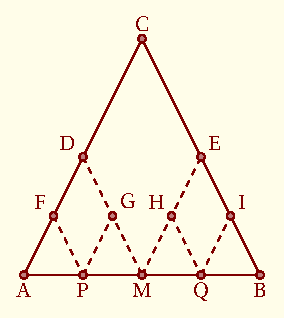
\includegraphics{10_home_antalcides_MEGA_calculo_I_libro_pdf_cal_lim8.pdf}
\caption{Sucesi\'on de puntos medios en un triángulo equilátero}
\label{fig:cal_lim8} \end{figure}

\end{ejemplo}

\sol La intuición nos indica que, cuando el número de lados del segmento
quebrado tienda a infinito su longitud tenderá a confundirse con la
longitud $l$ del segmento $AB;$ es decir, que el límite de la sucesión
de longitudes del segmento quebrado sería igual a $l.$ La demostración
de este hecho nos indicará que nuestra intuición no es correcta; en
efecto: la longitud del primer segmento quebrado, $ACB,$ es igual
a $2l;$ la de la segunda es $AD+DM+ME+EB=\frac{l}{2}+\frac{l}{2}+\frac{l}{2}+\frac{l}{2}=2l;$
análogamente, la longitud del tercer segmento quebrado y la de todas
las siguientes es igual a $2l$. Si representamos por $l_{n}$ la
longitud del n-ésimo segmento quebrado se cumple que $l_{n}=2l.$
para todo $n.$ La diferencia $\left\{ l_{n}-l\right\} =\left\{ 2l-l\right\} =\left\{ l\right\} $
no es infinitésima, y por tanto el límite de $\{l_{n}\}$ no es igual
a $l$, como la intuición nos indica.

El límite correcto es $2l,$ pues se tiene $\{ln-2l\}=\{2l-2l\}=\{0\},$
y una sucesión formada por ceros cumple con la definición de infinitésimo.\fin 

\general El límite de una sucesión cuyos términos son todos iguales
a una constante, $k,$ es igual a dicha constante; pues $\{k-k\}=\{0\}$
es una sucesión infinitésima. Insistimos en que el símbolo $\{0\}$
ha de interpretarse como una sucesión cuyos términos son todos ceros.
análogamente, el símbolo $\{k\},$ se interpreta como una sucesión
cuyos términos son todos iguales a $k.$

\begin{ejemplo}\label{ej:ejem8cv}

Consideremos la sucesión $\left\{ \dfrac{2n+1}{n+2}\right\} ,\text{\inline\text{\label{eq:ec2.8}.}}$
Sus primeros términos son: $\frac{3}{3},\;\frac{5}{4},\;\frac{7}{5},\;\frac{9}{6},\;\frac{11}{7},\cdots.$
Se observa que los términos de la sucesión se van acercando al valor
$2.$ Comprobemos si el valor $2$ es el límite de la sucesión infinitésima.

Se tiene: $\left\{ \dfrac{2n+1}{n+2}-2\right\} =\left\{ \dfrac{2n+1-2n-4}{n+2}\right\} =\left\{ \dfrac{-3}{n+2}\right\} \text{\inline\text{\label{eq:ec2.9}.}}$

Para probar que esta última sucesión es infinitésima habrá que probar
que, dado un $\epsilon>0,$ arbitrariamente pequeño, sus términos
son, en módulo, menores que $\epsilon,$ a partir de uno, es decir,
hay que probar que $\val{\dfrac{-3}{n+2}}<\epsilon$ para todo $n$
superior a un cierto valor; o sea, hay que probar que $\dfrac{3}{n+2}<\epsilon,\text{\inline\text{\label{eq:ec2.10},}}$
a partir de un $n;$ pero para que se cumpla la ecuación \ref{eq:ec2.10}
basta que $n+2>\frac{3}{\epsilon},$ o sea que $n>\frac{3}{\epsilon}-2;$
por tanto: la sucesión representada por la ecuación \ref{eq:ec2.9}
es infinitésima y la sucesión representada por la ecuación \ref{eq:ec2.8}
tiene por límite 2.

\end{ejemplo}

\begin{defi}{Límite finito}{def:limfi}

Se dice que una sucesión $\{a_{n}\},$ tiene por límite $\alpha,$
y se escribe $\Lim{a_n}{n}{\infty}=\alpha$ ó $a_{n}\to\alpha,$ si
y solamente sí, $\{a_{n}-\alpha\}$ es una sucesión infinitésima.

\end{defi}

\resu Las afirmaciones $\Lim{a_n}{n}{\infty}=\alpha$  y $\Lim{(a_n-\alpha)}{n}{\infty}=0$,
son equivalentes.\global\long\def\Lim#1#2#3{{\displaystyle \lim_{#2\to#3}}#1}

\noun{Expresión analítica}: $\Lim{a_{n}=\alpha,}n{\infty}$ si y solamente
sí, dado un $\epsilon>0,$ arbitrario, (en particular tan pequeño
como se quiera), se cumple que $\val{a_{n}-\alpha}<\epsilon$ para
todos los términos de la sucesión siguientes a uno dado.

Esta es la forma usual de presentar el concepto de límite en los textos
del Análisis Matemático; pero sin una preparación previa del lector,
le queda muy difícil comprenderla bien.

\noun{Interpretación Geométrica}: De acuerdo con lo explicado en el
ejemplo \myref{ej:ejem5cv} de la sección \ref{subsec:Interpretaci=0000F3n-geom=0000E9trica-de},
todos los números que verifican la relación modular $\val{a_{n}-\alpha}<\epsilon$
pertenecen al entorno de centro $\alpha$ y semi-amplitud $\epsilon.$

Pero la relación modular $\abs{a_{n}-\alpha}<\epsilon,$ (si $\alpha$
es el límite de $\{a_{n}\}$), la cumplen todos los términos de la
sucesión desde uno en adelante; por tanto concluimos que: $\alpha$
será el límite de $\{a_{n}\}$ si y solo sí, rodeando el punto $\alpha$
de un entorno, de semi-amplitud $\epsilon$ arbitrariamente pequeño,
tan pequeño como queramos, todos los términos de $\{a_{n}\}$ a partir
de uno en particular están dentro del entorno; por tanto: en el interior
de dicho entorno están infinitos puntos de la sucesión, y en el exterior
hay un número finito de puntos de $\{a_{n}\}$,

\begin{nota}\obs

No todas las sucesiones tienen límite. De acuerdo con lo afirmado
últimamente, el límite de una sucesión $\{a_{n}\}$ solo existe, cuando
existe un punto $\alpha$ que goza de la siguiente propiedad: En el
interior de cualquier entorno de $\alpha$, por pequeño que sea, existen
un número infinito de puntos de la sucesión $\{a_{n}\},$ y en el
exterior un número finito. Analíticamente; Los números que verifican
la condición $\alpha-\epsilon<a_{n}<\alpha+\epsilon$ son infinitos
y los que no son finitos.

\end{nota}

\begin{ejercicios}[]
\begin{enumerate}
\item Demostrar que el límite de $\left\{ \dfrac{3n+2}{n+1}\right\} $ es
igual a $3.$ (tome como orientación el ejemplo \ref{ej:ejem8cv}).
\item Demostrar que el límite de $\left\{ \dfrac{n^{2}+1}{n^{2}+9}\right\} $
es $1.$
\item Demostrar que el límite de $\left\{ \dfrac{n^{2}+1}{n^{2}}\right\} $
es $1.$
\item Demostrar que el límite de $\left\{ \dfrac{2n-1}{3n+1}\right\} $
es $\frac{2}{3}.$
\item Si se representa una sucesión $\{a_{n}\},$ con límite $\alpha,$
sobre un plano cartesiano, $\left(O_{n},O_{a_{n}}\right),$ y se trazan
las rectas paralelas al eje $O_{n},$ $y=\alpha-\epsilon$ y $y=\alpha+\epsilon,$
¿que puede decirse de los puntos de la sucesión a partir de uno en
particular? siendo $\epsilon>0$ un número cualquiera.
\item Si el límite de $\{a_{n}\}$ es $\alpha,$ ¿cuál será el límite de
$\{a_{n}+k\},$ siendo $k$ un número real constante? Haga un razonamiento
analítico de la situación y otro geométrico. 
\end{enumerate}
\end{ejercicios}

\section{Propiedades fundamentales de los límites.}

En esta sección desarrollaremos algunas propiedades fundamentales
de los límites que ilustran muy bien la parte esencial del concepto,
aparte de que algunas de tales propiedades serán usadas después, su
estudio dará oportunidad al lector de reafirmar bien el significado
exacto de la idea matemática de límite.

\begin{propiedad}{:\ Unicidad del límite}

Una sucesión no puede tener más de un límite.

\end{propiedad}

\begin{dems}

Supongamos que $\{a_{n}\}$ tiene dos límites distintos, $\alpha$
y $\beta$ como se observa en la figura \ref{fig:cal_lim10}. 

\begin{figure}[H] \centering

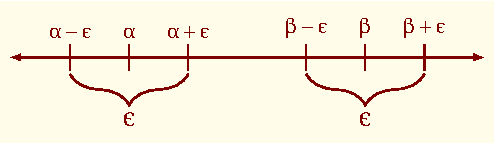
\includegraphics{11_home_antalcides_MEGA_calculo_I_libro_pdf_cal_lim10.pdf}
\caption{Unicidad del límite}
\label{fig:cal_lim10} \end{figure}

Elijamos un $\epsilon>0,$ menor que la mitad de la longitud $\val{\beta-\alpha}$;
si rodeamos los puntos de coordenadas $\alpha$ y $\beta$ de sendos
entornos de semi-amplitud $\epsilon,$ dichos entornos serán disjuntos.
Ahora, si $\{a\}$ tiene por límite $\alpha$ todos sus términos a
partir de uno valor dado, que representaremos por $a_{n_{1}},$ pertenecerán
al entorno de $\alpha;$ análogamente, si $\beta$ fuese también límite
de $\{a_{n}\}$ todos los términos de $\{a_{n}\},$ a partir de uno
que representaremos por $a_{n_{2}}$ pertenecerán al entorno de $\beta.$
Si consideramos los términos de $\{a_{n}\}$ siguientes a $a_{n_{1}}$
y $a_{n_{2}}$ dichos términos tendrían que pertenecer simultáneamente
al entorno de $\alpha$ y al de $\beta,$ lo cual es absurdo, ya que,
en virtud del postulado de Dedekind, cada término de $\{a_{n}\}$
(número real) solo tiene un punto correspondiente sobre la recta metrizada.\end{dems}

\begin{propiedad}{:\ Encaje}

Sean $\{a_{n}\},$ $\{b_{n}\}$ y $\{c_{n}\},$ tres sucesiones tales
que $a_{n}<c_{n}<b_{n}$ para todo $n:$ entonces si las sucesiones
$\{a_{n}\}$ y $\{b_{n}\}$ tienen el mismo límite, la sucesión $\{c_{n}\}$
tiene también el mismo límite. En otras palabras si una sucesión está
comprendida entre dos sucesiones que tienen el mismo límite, ella
tiene también el mismo límite.

\end{propiedad}

\begin{dems}

Sea $\Lim{a_{n}}n{\infty}=\Lim{b_{n}}n{\infty}=\alpha,$ Dado un $\epsilon>0$arbitrario,
en particular tan pequeño como queramos, si rodeamos el punto $\alpha$
de un entorno de semi-amplitud $\epsilon>0,$ se cumplirá:
\begin{enumerate}
\item Todos los puntos de $\{a_{n}\}$ a partir de un punto en particular,
que representaremos $a_{n_{1}}$estarán en el entorno de $\alpha.$
\item Todos los puntos de $\{b_{n}\}$ a partir de un punto en particular,
que representaremos $b_{n_{2}}$estarán en el entorno de $\alpha.$
\item Por tanto, todos los términos cuyo orden sea posterior a $n_{1}$
y a $n_{2},$ tanto de $\{a_{n}\}$como de $\{b_{n}\}$ estarán en
el entorno de $\alpha.$
\item En consecuencia, como todos los términos de $\{c_{n}\}$ cumplen que
$a_{n}<c_{n}<b_{n},$ se cumplirá que: todos los números de $\{c_{n}\}$
de orden posterior a $n_{1}$ y a $n_{2}$estarán en el entorno de
$\alpha,$y por tanto, $\alpha$ será el límite de $\{c_{n}\}.$
\end{enumerate}
\end{dems}

\begin{propiedad}{}

Sea $\Lim{a_{n}}n{\infty}=\alpha$ y $k$ un número real cualquiera
menor que $\alpha,$ $k<\alpha.$ Entonces, todos los términos de
$\{a_{n}\}$, a partir de un número dado son mayores que $k.$ (vea
la figura \ref{fig:cal_lim11} 

\end{propiedad}

\begin{figure}[H] \centering

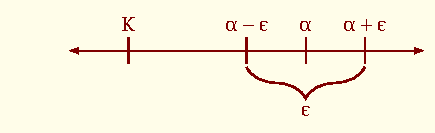
\includegraphics{12_home_antalcides_MEGA_calculo_I_libro_pdf_cal_lim11.pdf}
\caption{$a_n>k,\;\forall n$ tal que $k<\alpha $}
\label{fig:cal_lim11} \end{figure}

\begin{dems}

Elijamos un $\epsilon>0$ menor que la longitud $\val{\alpha-k}.$
Si rodeamos el punto $\alpha$ de un entorno de semi-amplitud $\epsilon,$
el punto $k$ quedará a la izquierda de dicho entorno; además, si
$\alpha$ es el límite de $\{a_{n}\},$ todos sus términos a partir
de un valor dado, estarán en el entorno de $\alpha$ y por tanto quedarán
a la derecha de $k$, es decir, serán mayores que $k.$ 

\end{dems}

Análogamente se demuestra que: si 

\section{Caso de límite infinito.}

\section{Sucesiones monótonas convergentes. }

\section{Ejemplos del principio del crecimiento limitado.}

\section{El límite fundamental de la sucesión.}

\section{Algunos problemas cuya solución depende del número $e.$}

\section{Las reglas de cálculo con infinitésimos. }
\end{document}
